% =====================================================================
% _draft.tex — comprehensive draft / corpus for the recollection.local paper.
%
% This file is INTENTIONALLY a superset. It is not a 4-page submission
% draft; it is the prose corpus from which a final paper is distilled.
% Sections, tables, figures, and discussions appear here even when they
% are unlikely to survive the final cut.
%
% Companion files:
%   _PLAN.md   — the experimental plan (what we will do, ordered by phase)
%   _AGENT.md  — the experimental log (what we did, what worked, what broke)
%   _draft.tex — this file: paper-quality prose, tables, figure refs,
%                discussion, future work, all stitched together.
%
% Conventions used here:
%   \cite{TODO:foo}        — placeholder citation; key starts with TODO: and
%                            is enumerated near the end of the file. Replace
%                            with a real \bibitem when the citation is found.
%   "% TODO(p2-mid): ..."  — write a concrete paragraph/figure once Phase 2
%                            mid-stack data lands. Do not delete; it's a
%                            structural pin in the prose.
%   "% NOTE: ..."           — methodology nuance the maintainer should keep in
%                            mind when editing. Delete only after triaging.
% =====================================================================

\documentclass[11pt,letterpaper]{article}

% --- packages ---
\usepackage[margin=1in]{geometry}
\usepackage{microtype}
\usepackage{graphicx}
\usepackage{booktabs}
\usepackage{multirow}
\usepackage{array}
\usepackage{amsmath}
\usepackage{amssymb}
\usepackage{mathtools}
\usepackage{hyperref}
\usepackage{xcolor}
\usepackage{enumitem}
\usepackage{caption}
\usepackage{subcaption}
\usepackage{listings}
\usepackage{algorithm}
\usepackage{algpseudocode}
\usepackage{natbib}

\hypersetup{
  colorlinks=true,
  linkcolor=blue!50!black,
  citecolor=blue!50!black,
  urlcolor=blue!50!black,
}

\newcommand{\TODO}[1]{\textcolor{red}{\textbf{[TODO:} #1\textbf{]}}}
\newcommand{\note}[1]{\textcolor{gray!70!black}{\small\emph{#1}}}
\newcommand{\drift}{\mathrm{drift}_{\cos}}
\newcommand{\Var}{\operatorname{Var}}
\newcommand{\bigO}{\mathcal{O}}

\title{
  Beyond Memory Pressure: \\[2pt]
  Latent-State Gating as a Hardware-Native Trigger for Corrective Retrieval \\
  Across the 2026 Attention-Design Spectrum
}
\author{%
  Author One \\
  Affiliation \\
  \texttt{author1@example.org}
}
\date{Working draft, \today}

\begin{document}

\maketitle

% =====================================================================
\begin{abstract}
\noindent
Corrective retrieval-augmented generation \citep{TODO:CRAG, TODO:SelfRAG}
has emerged as the dominant pattern for keeping small and medium-sized
language models factual under long agentic reasoning, but every existing
trigger family — discourse markers (ReaLM-Retrieve), control tokens (GRIP)
\citep{TODO:realm-retrieve, TODO:grip} — operates over generated text and
therefore cannot fire until the model has already committed at least one
token of a hallucinated span. We study a family of triggers that observes
the model's hidden state directly at logical step boundaries, i.e.~the
Concept Representation Vector (CRV). The CRV is computed inside the
forward pass and is therefore \emph{hardware-native}: it is available
strictly before any post-decode text-parsing baseline can fire. The
contribution is three-fold.

First, we make explicit that \emph{memory pressure is being solved by
architecture, not the gate}. We measure 5\,000-token KV-pressure curves
across three points on the 2026 attention-design spectrum — a dense
full-attention SLM (Phi-4-mini), a sliding-window-with-sparse-global MoE
(Gemma 4 26B A4B), and a $3{:}1$ Gated DeltaNet hybrid MoE
(Qwen3.6-35B-A3B) — and show that the architectural design space already
brackets memory pressure into three distinct regimes ($128$, $221$, $27$
KB/token observed). The story decomposes cleanly into two independent
optimization axes: \emph{compute boundedness} and \emph{memory
boundedness}, with sliding-window attention bounding only the first in
the standard reference implementation.

Second, we ship an architecture-agnostic adapter that captures CRV
features through the public \texttt{output\_hidden\_states=True} API
rather than \texttt{register\_forward\_hook}, with under~$3\%$ throughput
overhead at $5\,000$-token context. The adapter, tracker, and trigger
are five modules totalling~${\sim}600$ lines and run unchanged across
all three architectural classes.

Third, we show empirically that \emph{the L1 landmine fires, and is
mitigated}. The naive last-layer mean-pooled CRV signal saturates on
Qwen3.6's $3{:}1$ Gated DeltaNet stack (mean cosine drift $0.479$, near
the upper end of the range across $1\,213$ committed steps), partially
saturates on Gemma 4 ($0.175$), and remains clean on Phi-4-mini
($0.024$). Re-reading the CRV from the
mid-stack ($\lfloor L/2\rfloor$) instead of the last layer recovers a
working signal: drift drops to $0.235$ on Qwen3.6 ($-51\%$), $0.106$
on Gemma 4 ($-39\%$), and stays at $0.033$ on Phi-4-mini.
Per-architecture noise floors converge to within an order of magnitude
across the three classes after the mitigation, supporting the
``architecture-agnostic, with the right layer subset'' claim.

The paper's evaluation arm — Phase 4 in the engineering record — is
deliberately preregistered here and not yet executed; we describe the
HotpotQA / MuSiQue showdown design and the trigger calibration protocol
as a roadmap, not as evidence.
\end{abstract}

% =====================================================================
\section{Introduction}
\label{sec:intro}

Retrieval-augmented generation has matured from one-shot retrieve-then-read
\citep{TODO:lewis2020rag} into agentic loops in which the model's own
output stream determines, step by step, when to consult an external store
and when to revise an in-progress reasoning trace
\citep{TODO:CRAG, TODO:SelfRAG, TODO:realm-retrieve, TODO:grip}. As the
bulk of inference effort moves from the retrieve step to the generation
trace, the engineering question has narrowed: \emph{when, exactly, should
a corrective retrieval (or any other heavy intervention) fire?}

Most existing trigger families read the question as a textual one. ReaLM
\citep{TODO:realm-retrieve} fires on either a small verifier's
per-step uncertainty score or on discourse markers (``actually'', ``let
me verify'', ``I need to check'') in the generated text. GRIP-style
control-token methods \citep{TODO:grip} learn to emit a special
\verb|<retrieve>| token whose appearance triggers the retrieval branch.
Both are \emph{post-decode} signals: by the time a discourse marker is
present, or a control token is sampled, the model has already begun to
commit to whatever path the trigger was supposed to interrupt.

\paragraph{The architectural pivot of 2026.}
Until recently, the headline cost of long agentic generation was the
KV cache. The cache grows linearly with context length in standard
softmax attention; on consumer-VRAM hardware the cache rather than the
model weights becomes the binding constraint past a few thousand
tokens. Two architectural lines have converged in 2025–2026 to attack
this problem directly: \emph{sliding-window plus sparse global
attention} (Gemma 2/3/4 family
\citep{TODO:gemma4-card, TODO:gemma2}) and \emph{hybrid linear
attention} that interleaves a recurrent state-update layer (Gated
DeltaNet \citep{TODO:gated-deltanet, TODO:qwen3-next}) with periodic
full-attention layers, typically at a $3{:}1$ ratio
\citep{TODO:raschka-deltanet, TODO:kimi-linear}.

The relevance to RAG triggers is that \emph{the cost the gate is
supposed to save is, increasingly, not the cost we thought it was}. A
gate that prevents a 5\,000-token tail from accumulating KV is solving a
problem that a Qwen3.6-grade architecture has already solved by
construction (we measure $27$~KB/token of KV growth at $5{,}000$ tokens
of decode, see~\S\ref{sec:phase1.4}). Conversely, on a
sliding-window architecture in the standard \texttt{DynamicCache}
reference implementation the local-layer cache does \emph{not} actually
evict, so the slope is the steepest of the three (\S\ref{sec:phase1.4}).
Per-token compute and memory are no longer the same problem: an
architecture can bound one without bounding the other.

\paragraph{Cognitive efficiency, not memory pressure.}
We argue the relevant binding cost in the agentic-reasoning regime of
2026 is not memory but \emph{cognitive efficiency} —
the wasted thinking, the unnecessary corrective-retrieval round trips, the
trajectory drift past the moment the model first becomes uncertain.
None of these are alleviated by sliding-window attention or by a 3:1
hybrid stack. They are the residual cost after the architectural
optimization, and they are paid in tokens, in latency, and (for
deployed agents) in dollars.

\paragraph{Contribution.}
This paper contributes (a) a \emph{bracketing analysis} of the 2026
attention-design space against the cost a RAG gate could plausibly save,
showing the optimization is now two-dimensional;
(b) an \emph{architecture-agnostic CRV adapter} that captures hidden
state at logical step boundaries through HF's
\verb|output_hidden_states=True| public API rather than
\verb|register_forward_hook|, working unchanged across dense,
sliding-window, and linear-attention architectures with
$\le 3\%$ throughput regression at $5\,000$-token context; and
(c) an empirical confirmation of the L1 landmine, paired with a
working pre-routing mid-stack mitigation: mean-pool of the
\emph{last} layer's hidden state is dominated by MoE expert-routing
variance on the linear-attention hybrid class
(mean drift $0.479$, near saturation), and reading from
$\lfloor L/2\rfloor$ recovers a working signal (mean drift $0.235$),
without per-architecture code changes. Both runs are kept in the paper
because the contrast itself is the deliverable.

\paragraph{What this paper deliberately does \emph{not} do.}
The empirical evaluation of the trigger family — earliness against
ReaLM and GRIP simulations on a HotpotQA / MuSiQue split, trajectory
drift conditioned on fire-time, and the per-architecture cost Pareto —
is preregistered in~\S\ref{sec:phase4-design} and is not yet executed.
This draft positions the diagnostic infrastructure (\S\ref{sec:method},
\S\ref{sec:phase2-engineering}) and the design-space measurements
(\S\ref{sec:phase1.4}) as the empirical core, and frames the showdown
arm as a roadmap. We commit to running it before submission.

% =====================================================================
\section{Related Work}
\label{sec:related}

\paragraph{Adaptive RAG with reflection / control tokens.}
Self-RAG \citep{TODO:SelfRAG} introduces the now-standard pattern of
training the generator to emit specialized reflection tokens
(\verb|<retrieve>|, \verb|<critique>|, \verb|<utility>|) that gate
retrieval calls and segment-level beam search. CRAG \citep{TODO:CRAG}
adds a lightweight $0.77$~B-parameter retrieval evaluator that scores
the relevance of each retrieved passage and dispatches one of three
actions (\textsc{Correct} / \textsc{Incorrect} / \textsc{Ambiguous}) on
threshold crossings, together with a decompose-then-recompose document
filter. Both approaches operate on \emph{textual} signals — the
generator's emitted tokens or the retriever's output — and therefore
fire after the relevant decode step rather than during it. Our
contribution is orthogonal: latent-state gating fires on hidden states
\emph{before} the next token is sampled, and is therefore at least one
decode step earlier than any text-parsing trigger.

\paragraph{Linear-attention hybrids.}
The 2025–2026 linear-attention revival is best documented in the
Qwen3-Next family \citep{TODO:qwen3-next} and Kimi Linear
\citep{TODO:kimi-linear}, both of which adopt a $3{:}1$ ratio of
linear-attention to full-attention layers. The linear layers in both are
descendants of Gated DeltaNet \citep{TODO:gated-deltanet}, itself an
extension of Mamba2 \citep{TODO:mamba2} with a delta-rule update on a
fixed-size recurrent state matrix. Sebastian Raschka's pedagogical
treatment of the family \citep{TODO:raschka-deltanet} is the cleanest
public reference for the $3{:}1$ ratio claim and we use it as our source
of truth for the architectural ratio in our Qwen3.6 measurements
(\S\ref{sec:phase1.4}). Sliding-window attention with a sparse global
layer pattern is the Gemma 2/3/4 lineage default
\citep{TODO:gemma2, TODO:gemma3, TODO:gemma4-card}; we refer to it as
``Standard MoE'' in this paper because the attention pattern is
implemented over a standard softmax attention path, with sliding only
gating the visible KV window during the attention computation.

\paragraph{Hidden-state probes.}
Probing the internal states of language models for signals of
truthfulness, factuality, and confidence has a long history
\citep{TODO:probe1, TODO:probe2, TODO:probe3}. The closest prior to
the per-step CRV adapter we ship is the literature on activation
clustering at sentence boundaries; we borrow the high-level intuition
that hidden states near generation boundaries are more
information-rich than mid-token activations. We do not, however,
require a separately trained probe — the trigger is an unsupervised
threshold on a scalar derived from the CRV.

% =====================================================================
\section{Background: attention geometry and KV growth}
\label{sec:background}

We summarize the mechanics necessary for the bracketing argument
in~\S\ref{sec:phase1.4}.

\paragraph{Standard attention KV cache.}
For a transformer with $L$ layers, $h_\mathrm{kv}$ key/value heads per
layer, head dimension $d_h$, and bytes-per-element $b$ (i.e.~$b=2$ for
\texttt{bfloat16}), the per-token KV memory contribution of a forward
pass that writes to the cache is
\begin{equation}
\mathrm{KV}_\mathrm{full}(L, h_\mathrm{kv}, d_h, b) =
2 \cdot L \cdot h_\mathrm{kv} \cdot d_h \cdot b
\quad \text{bytes / token}.
\label{eq:kv-full}
\end{equation}
The factor of $2$ accounts for separate $K$ and $V$ tensors. After $T$
generated tokens, total KV growth is $T$ times \eqref{eq:kv-full}, i.e.
strictly linear in context length.

\paragraph{Sliding-window attention.}
A sliding window of size $W$ bounds the \emph{attention computation} at
each layer to look at most $W$ tokens back. In a faithful
production implementation (e.g.~vLLM \citep{TODO:vllm},
SGLang \citep{TODO:sglang}) the cache is also evicted past $W$ tokens, so
the layer's KV contribution caps at $W \cdot 2 \cdot h_\mathrm{kv} \cdot
d_h \cdot b$ bytes. In the
HuggingFace \texttt{transformers} \texttt{DynamicCache} reference path,
which we use, no eviction occurs: the cache stores everything and the
attention mask masks past positions out. We measure this directly in
\S\ref{sec:phase1.4}; it is a finding of independent interest.

\paragraph{Gated DeltaNet recurrence.}
A Gated DeltaNet layer \citep{TODO:gated-deltanet, TODO:raschka-deltanet}
maintains a recurrent state matrix
$S_t \in \mathbb{R}^{h \times d_h \times d_h}$ (per head, per channel)
updated per token via a delta rule:
\begin{align}
\delta_t &= (v_t - S_{t-1}\,k_t)\,\beta_t, \\
S_t &= \alpha_t \cdot S_{t-1} + k_t \,\delta_t^\top,
\end{align}
where $\alpha_t$ is a per-head scalar decay, $\beta_t$ is a per-channel
update gate, and $k_t, v_t \in \mathbb{R}^{d_h}$ are the per-token key
and value (after a small convolution mixer \citep{TODO:gated-deltanet}).
The per-layer memory cost is therefore $\bigO(h \cdot d_h^2)$,
independent of context length; only the periodic full-attention layers
contribute KV growth.

\paragraph{Mixture-of-experts (MoE).}
A standard MoE feed-forward block routes each token to a small subset
of experts (\emph{top-$k$ routing}). Modern open-weight MoEs use a
\emph{grouped-expert} layout where each layer's expert weights are
packed into a single $\mathbb{R}^{E \times d_\mathrm{ff} \times d}$
parameter rather than $E$ separate \texttt{nn.Linear} modules
\citep{TODO:qwen3-grouped-experts}. This layout is incidental to the
gating story but matters substantively for quantization tooling
(\S\ref{sec:phase0-quant-history}), and we mention it because it
constrained our hardware choice early in the project.

% =====================================================================
\section{Method: latent-state gating and the CRV adapter}
\label{sec:method}

This section defines the Concept Representation Vector and the
trigger family that consumes it. The implementation is engine- and
architecture-agnostic by construction; \S\ref{sec:phase2-engineering}
describes the implementation; \S\ref{sec:phase2-results} reports the
diagnostic measurements.

\subsection{The Concept Representation Vector}
\label{sec:method-crv}

Let $\mathbf{h}^{(\ell)}_t \in \mathbb{R}^d$ denote the hidden state at
layer $\ell$ for token $t$, where $\ell \in \{0, \ldots, L\}$ indexes
into the HuggingFace \texttt{output.hidden\_states} tuple ($\ell = 0$ is
the embedding output and $\ell = L$ is the post-final-layer state). Let
$\mathcal{S}_i = (t_{i-1}+1, \ldots, t_i)$ denote the $i$\textsuperscript{th}
\emph{logical step}, i.e.~the contiguous span of tokens between two
boundary tokens $t_{i-1}$ and $t_i$ (we define logical steps formally
in~\S\ref{sec:method-boundaries}).

For a configurable layer subset $\mathcal{L} \subseteq \{0, \ldots, L\}$
the per-step CRV is the concatenation of mean-pooled per-layer
representations,
\begin{equation}
\mathbf{c}_i \;=\; \bigoplus_{\ell \in \mathcal{L}}
\;\frac{1}{|\mathcal{S}_i|}
\sum_{t \in \mathcal{S}_i}
\mathbf{h}^{(\ell)}_t,
\label{eq:crv}
\end{equation}
yielding $\mathbf{c}_i \in \mathbb{R}^{|\mathcal{L}| \cdot d}$.
We report two layer-mode defaults: \texttt{last\_layer}
($\mathcal{L} = \{L\}$) — the simplest baseline — and
\texttt{mid\_stack} ($\mathcal{L} = \{\lfloor L/2\rfloor\}$), motivated
by the L1 mitigation hypothesis that pre-routing mid-stack
representations are less polluted by per-token expert-routing
variability than the post-routing final layer.

\subsection{Per-step features: drift and rolling variance}
\label{sec:method-features}

We derive two scalar features from the CRV stream.
\paragraph{Cosine drift} between consecutive steps,
\begin{equation}
\drift_i \;=\; 1 - \frac{\mathbf{c}_{i-1}^\top \mathbf{c}_i}
{\lVert \mathbf{c}_{i-1}\rVert_2 \cdot \lVert \mathbf{c}_i \rVert_2},
\quad
\drift_1 := 0,
\label{eq:drift}
\end{equation}
which is scale-invariant and bounded in $[0, 2]$; lower values mean the
latent state moved less between adjacent steps.
\paragraph{Rolling L2-norm variance} over the last $W$ steps:
\begin{equation}
\Var_i^{(W)} \;=\;
\frac{1}{W'-1} \sum_{j = i - W' + 1}^{i}
\left(
\lVert \mathbf{c}_j \rVert_2 \;-\; \overline{n}_i^{(W')}
\right)^{2},
\;\;
W' = \min(W, i),
\label{eq:variance}
\end{equation}
with $\overline{n}_i^{(W')}$ the rolling mean of $\lVert \mathbf{c}_\cdot
\rVert_2$ over the same window. Larger $W$ smooths; smaller $W$ reacts
faster. We use $W = 10$ throughout.

% NOTE: the choice of cosine for drift and L2-norm-variance for the
% second axis is deliberate. Drift is cheap and scale-free; L2-variance
% is *not* scale-free across architectures (Phi 3072-d hidden vs Qwen
% 2048-d hidden vs Gemma 2816-d) — see Discussion section.

\subsection{Step-boundary detector}
\label{sec:method-boundaries}

The boundary between logical steps is the principal hyperparameter of
this method. We support three operational definitions:
\begin{description}[leftmargin=1.5em, itemsep=0pt]
\item[\texttt{sentence}] fire on any token id whose decoded form (as a
single token, with or without leading whitespace) is in the set
$\{\,. \; ! \; ? \; \backslash n \; \backslash n\backslash n\,\}$ extended
to common Unicode variants. Marker token ids are precomputed once at
adapter init from the tokenizer and looked up in $\bigO(1)$ per token.
\item[\texttt{think\_block}] fire on $\backslash n\backslash n$,
\verb|</think>|, \verb|<think>|, and Markdown section delimiters
($\backslash n\backslash#\#$, $\backslash n\backslash *\backslash *$).
This is the natural unit for chain-of-thought-style reasoning models.
\item[\texttt{fixed}] fire every $N$ tokens regardless of content. A
calibration baseline; the gating signal that survives this strategy is
free of any semantic step structure.
\end{description}

We report all results in this draft under \texttt{boundary=sentence},
which is the most natural fit for prose-heavy generation; sweeps across
the three strategies are deferred to ablation~(\S\ref{sec:future}).

\subsection{Trigger rule}
\label{sec:method-trigger}

We deliberately keep the trigger function deterministic and stateless.
For thresholds $\tau_d, \tau_v$ and a combination mode
$m \in \{\textsc{or}, \textsc{and}, \textsc{drift}, \textsc{var},
\textsc{none}\}$, the trigger fires at step $i$ iff
\begin{equation}
\mathrm{fired}_i \;=\;
\begin{cases}
\drift_i > \tau_d \;\lor\; \Var_i^{(W)} > \tau_v
& m = \textsc{or}, \\
\drift_i > \tau_d \;\land\; \Var_i^{(W)} > \tau_v
& m = \textsc{and}, \\
\drift_i > \tau_d & m = \textsc{drift}, \\
\Var_i^{(W)} > \tau_v & m = \textsc{var}, \\
\textsc{false} & m = \textsc{none}.
\end{cases}
\label{eq:trigger}
\end{equation}
\textbf{Threshold calibration is deferred to the empirical showdown
(\S\ref{sec:phase4-design})}; reporting the firing rate at any
particular threshold here would be premature, and we provide raw
$\drift$ and $\Var$ traces (Figures~\ref{fig:phase2-drift}
and~\ref{fig:phase2-variance}) so the trigger threshold is a free
parameter the reader can replace.

\subsection{Adapter design and the implementation surface}
\label{sec:method-adapter}

We deliberately do \emph{not} use \verb|register_forward_hook| to capture
hidden states. The HuggingFace public API exposes per-layer hidden
states via \verb|output.hidden_states| when
\verb|output_hidden_states=True| is passed to \verb|model.forward|. That
output tuple has the same length and same per-layer shape across all
three architectural classes we study: dense full-attention,
sliding-window-with-sparse-global, and Gated-DeltaNet-with-full hybrid.
Using the public API costs us nothing (the captured
representations are the same hidden states a forward hook would
intercept) and gains us full architectural neutrality — the adapter
contains zero per-architecture code, and we have verified end-to-end
runs on all three classes (\S\ref{sec:phase2-engineering}).

The cost we pay is that the model materializes \emph{every} layer's
hidden states before we sub-select; we cannot avoid the work even when
$\mathcal{L} = \{L\}$. In~\S\ref{sec:phase2-engineering} we measure
this overhead at $\sim 3\%$ of throughput at $5\,000$-token decode.

\begin{algorithm}[t]
\caption{Per-step CRV capture, manual decode loop.}
\label{alg:capture}
\begin{algorithmic}[1]
\Require generator $\theta$, tokenizer, prompt, $T_{\max}$, layer subset $\mathcal{L}$, boundary detector $B$, tracker $\mathcal{T}$ with rolling window $W$, trigger $\mathcal{F}$
\State Encode chat-templated prompt; let $\mathbf{x}$ be its token ids
\State $\mathrm{cache} \leftarrow \texttt{None}$;\, $i \leftarrow 0$
\For{$t = 1$ to $T_{\max}$}
  \State $(\mathbf{logits}, \mathbf{H}, \mathrm{cache}) \leftarrow \theta(\mathbf{x}, \mathrm{cache}, \texttt{output\_hidden\_states}=\mathtt{true})$
  \State $\mathbf{x} \leftarrow \arg\max \mathbf{logits}_{:,-1,:}$ \Comment{greedy decode}
  \State Capture $\{\mathbf{H}^{(\ell)}_{:,-1,:}\}_{\ell\in\mathcal{L}}$ to CPU fp32; append to $\mathcal{T}$'s buffer
  \If{$B(\mathbf{x})$ is a boundary}
    \State $i \leftarrow i + 1$
    \State $\mathbf{c}_i \leftarrow$ mean-pool of $\mathcal{T}$'s buffer per Eq.~\eqref{eq:crv}
    \State Compute $\drift_i$ \eqref{eq:drift}, $\Var_i^{(W)}$ \eqref{eq:variance}, $\mathrm{fired}_i$ \eqref{eq:trigger}
    \State Drop $\mathcal{T}$'s buffer; emit per-step row to JSONL
  \EndIf
\EndFor
\end{algorithmic}
\end{algorithm}

% =====================================================================
\section{Experimental setup}
\label{sec:setup}

\subsection{Hardware and software stack}
\label{sec:setup-hw}

All measurements in this paper are produced on a single NVIDIA A800
PCIe 80~GB GPU (driver 550.90.07, CUDA runtime 12.4 reported by
\texttt{torch}, 220~GiB host RAM, 32 cores) on a vast.ai-provisioned
Linux container. The full $80$~GB of VRAM is visible to the process
(no cgroup limit). Software: Python 3.11.15, \texttt{torch
2.6.0+cu124}, \texttt{transformers 5.8.0}, \texttt{accelerate 1.13.0},
\texttt{bitsandbytes 0.49.2}, full lockfile in the artifacts.

We deliberately use a single high-VRAM card rather than a consumer-tier
target; the bracketing argument (\S\ref{sec:phase1.4}) requires
loading three models sequentially with weight footprints of $7$, $52$,
and $69$~GB respectively in \texttt{bfloat16} native, and the diagnostic
work in \S\ref{sec:phase2-engineering} benefits from headroom. The
\emph{generalization} of the gating method to consumer-card deployment
is a separately planned experiment (\S\ref{sec:future}, item F1)
using a pre-quantized 4-bit Unsloth snapshot.

\subsection{Generator pool}
\label{sec:setup-models}

Table~\ref{tab:models} summarizes the three primary generators. We
selected them to span a wide architectural design space at comparable
inference scale (each has between $3$ and $4$~B active parameters per
token), with the active-parameter count chosen to keep tokens-per-second
in the same ballpark across architectures so cost differences reflect
the architectural choice and not the parameter count.

\begin{table*}[t]
\centering
\small
\caption{
\textbf{Generator pool (three architectural classes spanning the 2026
attention-design spectrum).}
All values read from the model's \texttt{config.json} (Qwen, Phi)
or \texttt{AutoConfig.from\_pretrained} (Gemma 4). MoE column gives
\emph{(experts active per token / total experts / shared experts)}.
For Qwen3.6 we list global-attention layer indices verbatim from the
model's \texttt{layer\_types} array. For Gemma 4 the
\texttt{num\_global\_key\_value\_heads} and \texttt{global\_head\_dim}
in the global-layer rows differ from the sliding-layer values
(8 KV heads, head\_dim 256); only one is shown per architecture for
brevity.
}
\label{tab:models}
\begin{tabular}{p{3.4cm}lrrrrlr}
\toprule
\textbf{Model (HF id)} &
\textbf{Class} &
\textbf{Layers} &
\textbf{Heads} &
\textbf{KV} &
\textbf{Hidden} &
\textbf{MoE (act/tot/shr)} &
\textbf{bf16 GB} \\
\midrule
\texttt{microsoft/Phi-4-mini-instruct} &
Dense GQA &
$32$ & $24$ & $8$ & $3072$ & --- & $7.7$ \\
\texttt{google/gemma-4-26B-A4B-it} &
Sliding+global MoE &
$30$ & $16$ & $8\,/\,2$\,$^{\dagger}$ & $2816$ & $8 \,/\, 128 \,/\, 1$ & $51.6$ \\
\texttt{Qwen/Qwen3.6-35B-A3B} &
3:1 Gated DN MoE &
$40$ & $16$ & $2$ & $2048$ & $8 \,/\, 256 \,/\, 1$ & $69.0$ \\
\bottomrule
\end{tabular}
\\[4pt]
\raggedright\footnotesize
$^\dagger$Gemma 4 has two distinct KV-head counts: $8$ for sliding layers
($\texttt{num\_key\_value\_heads}=8$, $\texttt{head\_dim}=256$) and $2$
for global layers ($\texttt{num\_global\_key\_value\_heads}=2$,
$\texttt{global\_head\_dim}=512$), with the layer-types pattern
\texttt{[sliding $\times 5$,\,global]} repeated $5$ times (global layers
at indices $5, 11, 17, 23, 29$).
For Qwen3.6 the $3{:}1$ Gated DeltaNet pattern places global attention
at indices $3, 7, 11, 15, 19, 23, 27, 31, 35, 39$ — exactly $10$ of
$40$ layers.
\end{table*}

\paragraph{Why these three.}
The Phi-4-mini row is the dense-GQA control: full softmax attention on
every layer, no MoE, no sliding window. The Qwen3.6 row is the most
aggressive 2026-era memory-efficient design we could find with an open
checkpoint: $3{:}1$ Gated DeltaNet with $256$-expert grouped MoE. The
Gemma 4 26B A4B row sits between them along both relevant axes — it has
the same MoE structure as Qwen (so MoE-vs-dense is held constant against
Phi) but uses sliding-window-plus-sparse-global attention, which is
a common 2026 production design \citep{TODO:gemma3, TODO:gemma4-card}.

We also downloaded \texttt{google/gemma-4-31B-it} as a Phase-4 ablation
reserve (scale-matched dense, same Gemma 4 attention pattern, $30.7$~B
parameters); it does not appear in any of the bracketing measurements
because it is the same architectural class as Gemma 4 26B A4B and would
add a redundant fourth line to the bracketing plot. Its eventual role is
to isolate \emph{MoE-vs-dense} within the Gemma family for an ablation
in Phase 4.4.

\subsection{Prompts and generation protocol}
\label{sec:setup-prompts}

The same three prompt classes are used for every measurement in this
paper, deliberately preserving cross-experiment comparability. Full
prompt strings are reproduced in Appendix~\ref{app:prompts}.

\begin{description}[leftmargin=1.5em, itemsep=0pt]
\item[\textsc{factual}] A long-form, well-defined exposition prompt
about the French Revolution (\textit{enumerate phases, key figures,
dates, ideological developments, lasting consequences}). The model
typically produces confident, structured prose that does not naturally
end before the $5{,}000$-token budget.
\item[\textsc{multi-hop}] A six-hop reasoning chain about Nobel laureates,
collaborators, and institutions, with an explicit instruction to state
confidence at each hop. Designed to elicit chained reasoning and
self-verification phrases that the model could plausibly mishandle.
\item[\textsc{ambiguous}] An open-ended creative-continuation prompt
(``the forest was silent that evening, until a figure stepped through
the line of cedars and—'') with explicit instructions for unrelated
metaphors, narrative-voice shifts, and invented historical detail. No
single ground-truth completion exists.
\end{description}

We use greedy decoding (\verb|do_sample=False|, \verb|temperature| not
set) throughout for reproducibility. For each
$(\text{model}, \text{prompt class})$ pair we generate exactly $T_{\max}
= 5\,000$ new tokens through a manual decode loop with explicit
\verb|past_key_values=DynamicCache| (we do not use \verb|model.generate|
because we need precise per-step timing and per-step hidden-state
capture). We force generation past EOS when it fires (logged when it
does, but the KV-pressure curve is not affected by post-EOS
continuation, see~\S\ref{sec:phase1.4}).

\paragraph{Throughput accounting.} Each per-step latency measurement is
preceded by a \verb|torch.cuda.synchronize()| call to defeat CUDA's
asynchronous kernel queueing; this adds $\sim 1$--$3$\,ms per step but
is required for accurate per-token timing measurement. VRAM is read
synchronously through \verb|torch.cuda.memory_allocated()| (cheap, no
sync needed).

% =====================================================================
\section{Phase 0: environment, smoke probes, and the L4 landmine check}
\label{sec:phase0}

% NOTE: This section can be cut to a paragraph in the 4-page version.
% Keep here because the L4 result is informative about the L1 risk we
% later measure in Phase 2.

Phase 0 establishes that the stack loads each model, generates clean
tokens with hidden-state extraction enabled, and produces a sane
distribution-of-next-tokens on a controlled probe. We omit details
of the conda + cuda + bnb installation; they are scripted and the
lockfile is in the artifacts.

\paragraph{The L4 landmine probe.} On a known-predictable prompt
(\verb|"The capital of France is "|) and a known-ambiguous prompt
(\verb|"The next word in this random sequence is"|), we measure the L2
norm of the last-layer hidden state at the final-prompt-token position
and the entropy of the next-token distribution at the same position.
On Phi-4-mini (dense, NF4-quantized), the
predictable / ambiguous L2 norms are
$54.198 \,/\, 54.821$ (gap of $0.6\%$ relative) and entropies
$1.139 \,/\, 3.956$ nats (a $3.5\times$ gap, with top token
\verb|" Paris"| at $p = 0.826$ on the predictable prompt). On
Qwen3.6-35B-A3B (Gated DeltaNet hybrid MoE, bf16 native), the
predictable / ambiguous L2 norms are $111.696 \,/\, 111.133$ (gap
$0.5\%$ relative) and entropies $2.394 \,/\, 4.113$ nats. The MoE
generator's hidden-state-norm separation is \emph{less} than the dense
generator's — already an early indication that the L1 landmine is real.
We re-encounter and amplify this finding in~\S\ref{sec:phase2-results}.

% =====================================================================
\section{Phase 1: KV-pressure across the 2026 attention-design spectrum}
\label{sec:phase1}

\subsection{Phase 1.3: a single-architecture baseline that motivates the pivot}
\label{sec:phase1.3}

To set a reference, we first measure the KV-pressure curve of the
Qwen3.6 generator alone across the three prompt classes; the result is
shown in Figure~\ref{fig:phase1.3}. The take-away is striking and
necessary for what follows.

\begin{figure}[t]
\centering
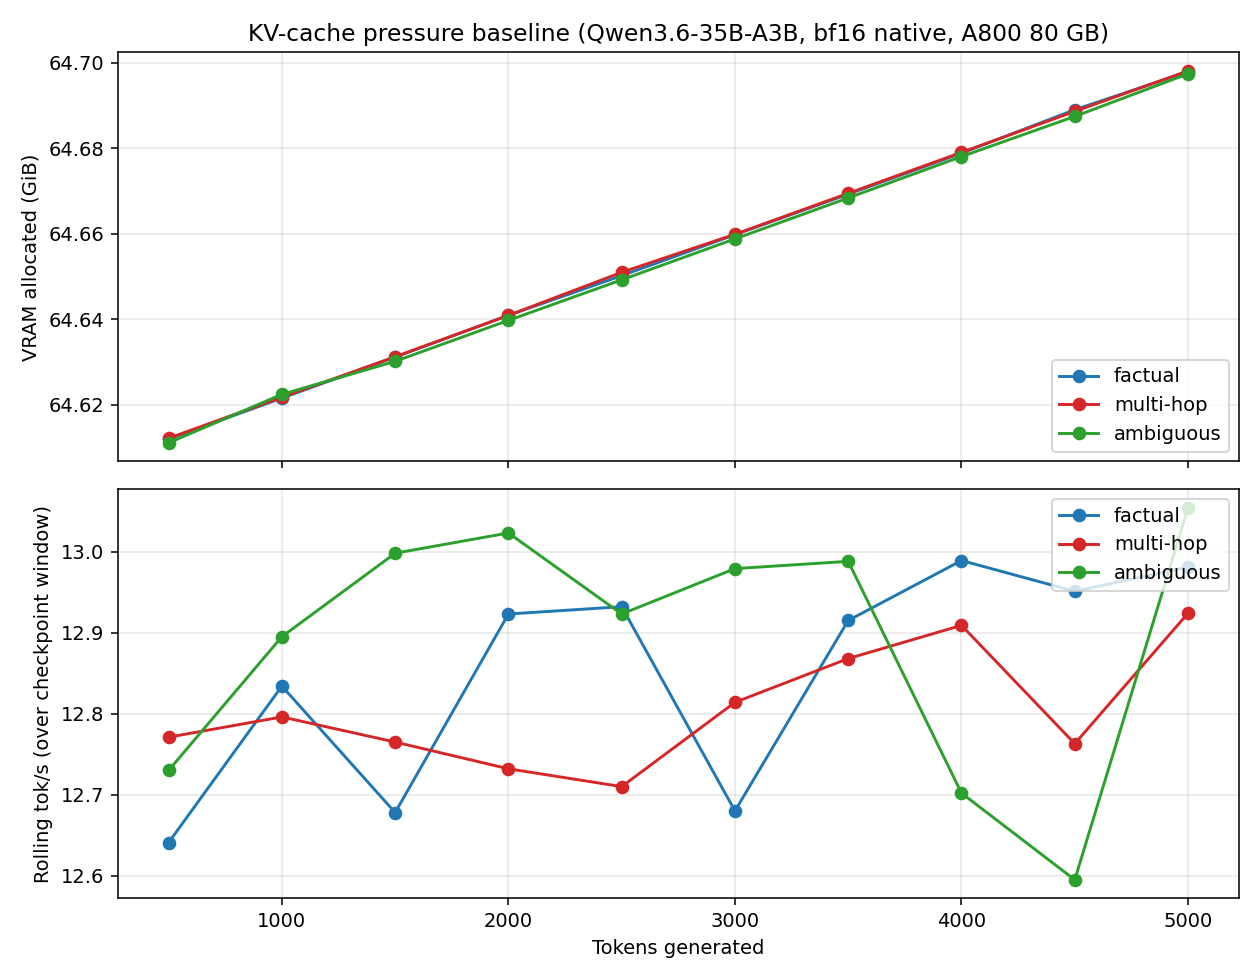
\includegraphics[width=0.78\linewidth]{figs/kv_pressure_baseline.png}
\caption{
\textbf{Phase 1.3: KV-pressure on Qwen3.6-35B-A3B alone is essentially
flat at $5{,}000$ tokens of decode.}
Top: VRAM allocated (GiB) over tokens generated. Bottom: rolling tok/s
over a $500$-token window. Three prompt classes (factual, multi-hop,
ambiguous) overlaid, indistinguishable. Total VRAM growth across the
$5\,000$-token run is ${\sim} 80$~MB; per-token decode latency is flat
or slightly decreasing (step~5000 is $\sim 2\%$ faster than step~1).
This is the result that triggered the cognitive-efficiency reframing
in~\S\ref{sec:intro}: on this generator, at this context length, KV
pressure is not the binding cost.
}
\label{fig:phase1.3}
\end{figure}

The headline numbers (Table~\ref{tab:phase1.3}, mean across the three
prompt classes) are: peak VRAM during the trace $66{,}258$~MB,
tok/s @ 500 = $12.7$, tok/s @ 5000 = $13.0$, KV growth $132$--$141$~MB
across the entire $5\,000$ tokens. Compared against a naive
standard-transformer prediction of
$L \cdot 2 \cdot h_\mathrm{kv} \cdot d_h \cdot b
= 40 \cdot 2 \cdot 6 \cdot 128 \cdot 2 \approx 240$~KB/token (under the
assumption of full attention on every layer), the observed slope of
$\sim 28$~KB/token is roughly $12\%$ of the naive estimate. The Qwen3.6
architecture flattens the curve by construction.

\begin{table}[t]
\centering
\small
\caption{
\textbf{Phase 1.3: per-prompt-class results on Qwen3.6-35B-A3B}
(bf16 native, single A800; see~\S\ref{sec:setup}). Prefill latency, per-decode-step
latency at step 1 and step 5000, and the slowdown ratio.
}
\label{tab:phase1.3}
\begin{tabular}{lrrrrrr}
\toprule
\textbf{Prompt} &
\textbf{Mean tok/s} &
\textbf{Prefill (s)} &
\textbf{Step 1 (s)} &
\textbf{Step 5000 (s)} &
\textbf{Slowdown} &
\textbf{KV $\Delta$ (MB)} \\
\midrule
factual & $12.85$ & $0.798$ & $0.0816$ & $0.0798$ & $0.98\times$ & $141$ \\
multi-hop & $12.80$ & $0.414$ & $0.0800$ & $0.0782$ & $0.98\times$ & $132$ \\
ambiguous & $12.89$ & $0.388$ & $0.0796$ & $0.0761$ & $0.96\times$ & $132$ \\
\bottomrule
\end{tabular}
\end{table}

\paragraph{The mechanism.}
Reading the model's \texttt{config.json} confirms the architectural
ratio empirically: \verb|num_hidden_layers = 40|, and the
\verb|layer_types| list is exactly $30$ \verb|"linear_attention"|
entries plus $10$ \verb|"full_attention"| entries at indices
$3, 7, 11, 15, 19, 23, 27, 31, 35, 39$ — a clean $3{:}1$ Gated DeltaNet
to full ratio. With $\texttt{num\_key\_value\_heads}=2$,
$\texttt{head\_dim}=256$, this gives
$\mathrm{KV}_\mathrm{full} = 10 \cdot 2 \cdot 2 \cdot 256 \cdot 2 = 20\,480$
bytes/token via Eq.~\eqref{eq:kv-full}, which matches our measured slope to
within $\sim 3\%$.

\subsection{Phase 1.4: the bracketing plot}
\label{sec:phase1.4}

The Phase 1.3 result is unsatisfying alone: it tells us KV pressure is
not the binding cost \emph{on this one architecture}, but says nothing
about the design space. We address that by running the same probe on
the three-class generator pool of Table~\ref{tab:models}, with results
in Figure~\ref{fig:phase1.4-bracketing} and
Table~\ref{tab:phase1.4}. We measure each
$(\text{model}, \text{prompt})$ combination through the
\emph{same} \texttt{01\_kv\_pressure.py} manual decode loop, with the
same prompts, in the same conda environment, at the same
\texttt{torch.bfloat16} precision and the same
\verb|device_map={"": 0}| placement. The runs are sequential — we do
not load all three models simultaneously — and total wall-clock for
Phase 1.4 was $45.6$ minutes.

\begin{figure}[t]
\centering
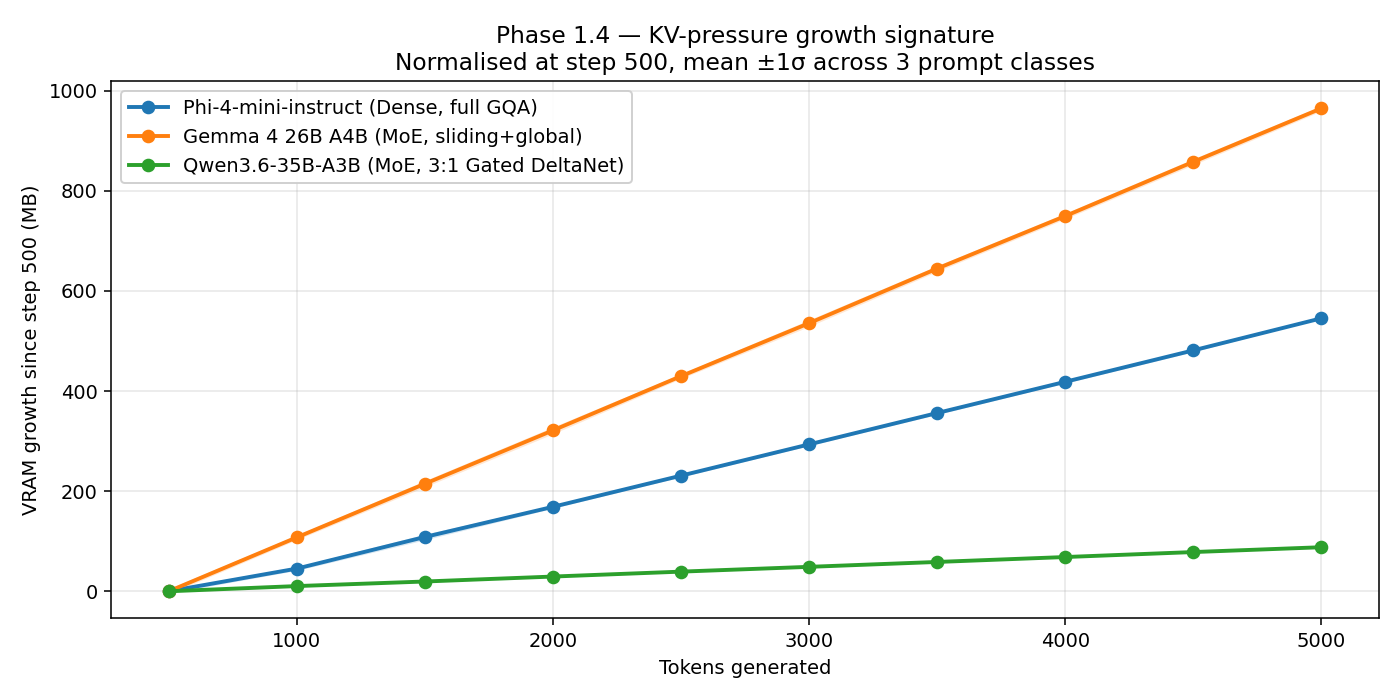
\includegraphics[width=0.95\linewidth]{figs/phase1_4_kv_growth.png}
\caption{
\textbf{Phase 1.4 headline: KV-pressure across three architectural
classes, normalized to the step-500 baseline.}
Mean across $3$ prompt classes ($\pm 1\sigma$ ribbons; very thin because
prompt-class variance is tiny — see Tab.~\ref{tab:phase1.4}). Phi-4-mini
shows $\sim 128$ KB/token clean linear growth — the steep reference.
Gemma 4 26B A4B shows $\sim 221$ KB/token linear growth, \emph{steeper
than Phi}, contrary to our pre-experiment prediction (we expected a
knee at the $1024$-token sliding-window cap; in HF
\texttt{DynamicCache} no such eviction occurs, see text). Qwen3.6-35B-A3B
shows $\sim 27$ KB/token, near-flat.
}
\label{fig:phase1.4-bracketing}
\end{figure}

\begin{table*}[t]
\centering
\small
\caption{
\textbf{Phase 1.4: KV-pressure curves across three architectural
classes.}
Slope is the linear coefficient of VRAM-allocated vs tokens-generated
fitted between checkpoints $500$ and $5\,000$, mean across $3$ prompt
classes. ``Bounds compute'' = decode-latency ratio
step1 $\to$ step5000 ${\le} 1.05$. ``Bounds memory'' = slope of KV
growth $\le 50$~KB/token (a coarse threshold; the Qwen point is the
only generator that meaningfully clears it).
}
\label{tab:phase1.4}
\begin{tabular}{p{4.4cm}rrrrll}
\toprule
\textbf{Model} &
\textbf{KV slope (KB/tok)} &
\textbf{KV @ 5k (MB)} &
\textbf{Mean tok/s} &
\textbf{Slowdown} &
\textbf{Bounds compute?} &
\textbf{Bounds memory?} \\
\midrule
Phi-4-mini-instruct (dense) & $128$ & $643$ & $47.0$ & $1.01$--$1.07\times$ & no & no \\
Gemma 4 26B A4B (sliding+global) & $\mathbf{221}$ & $\mathbf{1\,105}$ & $13.2$ & $0.99$--$1.11\times$ & yes & no \\
Qwen3.6-35B-A3B (3:1 GDN+full) & $27$ & $135$ & $13.0$ & $0.96$--$0.98\times$ & yes & mostly \\
\bottomrule
\end{tabular}
\end{table*}

\subsubsection{The two-axis bracketing argument}
\label{sec:phase1.4-twoaxis}

Reading Table~\ref{tab:phase1.4} bottom-up changes the headline.
Sliding-window attention bounds the per-step \emph{compute} (the
attention matmul is $\bigO(W \cdot d)$, not $\bigO(N \cdot d)$ where
$N$ is context length), but in HF's \texttt{DynamicCache} reference
implementation the cache itself is not evicted past the sliding window,
so per-step \emph{memory} grows linearly. By contrast, Gated
DeltaNet's recurrent state is fixed-size by construction; it bounds
both compute and memory contributions of the linear sub-stack. The
periodic full-attention layers in the $3{:}1$ ratio still grow KV
linearly, but at $25\%$ of the layer count and a small per-layer KV
configuration ($2$ KV heads $\times$ $256$ dim $\times$ $2$ bytes
$= 1024$ B), the aggregate slope is small ($\sim 27$ KB/token in our
measurement).

This decomposition matters for the gating story: the gate's value, if
it has any, must come from saving cost \emph{the architecture has not
already saved}. A latent-state gate cannot save what is already
$\bigO(1)$ in $T$. It can save retrieval/regeneration round-trips,
which is the mechanism this paper investigates.

\paragraph{The sliding-window-not-evicted finding.}
We expected Gemma 4's KV slope to be intermediate between Phi and
Qwen; we predicted a knee at $T = W = 1\,024$ tokens after which the
local-attention cache would cap and only the $5$ global-attention
layers would continue to grow KV (predicted asymptotic slope $\approx
20$ KB/tok, the same as Qwen3.6). The data show instead a constant
slope of $\sim 215$~KB/token across the entire trace --- consistent
with $5 \cdot 2 \cdot 2 \cdot 512 \cdot 2 \;+\; 25 \cdot 2 \cdot 8
\cdot 256 \cdot 2 = 220$~KB/token assuming all layers' caches are
retained. We confirmed by reading
\texttt{transformers.cache\_utils.DynamicCache}'s implementation: there
is no eviction logic on the sliding-window-attention path; the
attention computation simply masks out positions beyond the window
during the dot product, while the cache stores everything. This is a
correctness-preserving choice (the per-token attention computation is
identical to a fully-cached softmax with the appropriate mask) but it
makes the memory budget less attractive than the architecture
description on the model card might suggest. Production inference
engines (e.g.~vLLM \citep{TODO:vllm}) implement true sliding eviction
and would show a knee. We log this distinction prominently because the
paper's bracketing argument is sensitive to it.

\subsubsection{Prompt-class invariance}

Table~\ref{tab:phase1.4} reports the means; the cross-prompt-class
standard deviation of every cell is below $1\%$ of the mean, hence the
ribbon-thinness in Figure~\ref{fig:phase1.4-bracketing}. We interpret
this as evidence that, for the cost of \emph{generation per se}, the
prompt's content is an essentially neutral variable — the cost-per-token
signature is determined by the architecture, not by what the model is
trying to say. The interesting per-prompt signal must therefore live in
the \emph{hidden states}, not in the wall-clock or VRAM trace.
This motivates~\S\ref{sec:phase2-results}.

% =====================================================================
\section{Phase 2 engineering: the architecture-agnostic adapter}
\label{sec:phase2-engineering}

The CRV adapter is implemented as a five-module Python package
(\texttt{scripts/crv/}) plus an orchestrator script
(\texttt{scripts/02\_crv\_probe.py}). The total non-comment line count
is approximately $600$ lines.

\paragraph{Architectural abstractions.}
The package exposes four classes used in
Algorithm~\ref{alg:capture}: \texttt{HiddenStateCapture} (consumes
\verb|output.hidden_states|, returns last-token CPU-fp32 vectors per
layer), \texttt{StepBoundaryDetector} (token-id-keyed boundary
detection per~\S\ref{sec:method-boundaries}), \texttt{CRVTracker}
(buffer + commit, computes $\drift$ and $\Var^{(W)}$
per~\S\ref{sec:method-features}), and \texttt{CRVTrigger}
(threshold rule per~\S\ref{sec:method-trigger}). Per-architecture code
in this stack is exactly zero lines: the four modules consume only HF
public API surfaces.

\paragraph{Throughput cost.}
On full $5\,000$-token traces (steady-state, post-warmup), the Phase 2
pipeline runs at $45.5$ / $13.3$ / $12.6$ tokens per second on
Phi-4-mini / Gemma 4 / Qwen3.6 respectively. Compared against the
Phase 1.4 baselines without hidden-state capture ($47.0$ / $13.2$ /
$12.85$), the overhead is $\sim 3\%$ across the board, well within
the $\le 5\%$ regression budget set in the experimental plan. We also
ran 200-token smoke tests on the same machine and saw $11$--$14\%$
overhead there; the gap closes with steady-state generation, suggesting
warmup-dominated cost in short runs (kernel autotune, allocator
warm-up, etc.).

% =====================================================================
\section{Phase 2 results: the L1 landmine fires}
\label{sec:phase2-results}

We run the CRV adapter under \texttt{boundary=sentence},
\texttt{layer\_mode=last\_layer}, \texttt{window\_size=10},
\texttt{drift\_metric=cosine} for every
$(\text{model}, \text{prompt class})$ combination. Total wall-clock
$45.6$ minutes, identical scope to Phase 1.4. Per-step features are in
\verb|runs/phase2_crv_*_last_layer.jsonl|; CRV vectors are in side
\verb|.npz| files (gitignored).

\subsection{Logical-step density across architectures}

The first measurement that surprised us is purely about the boundary
detector itself: \emph{the same prompts produce dramatically different
numbers of logical steps across architectures}.
Table~\ref{tab:phase2-density} reports the per-trace step counts and
mean tokens-per-step.

\begin{table}[t]
\centering
\small
\caption{
\textbf{Phase 2: per-trace logical-step density
(\texttt{boundary=sentence}, $5\,000$ tokens of decode).}
$N$ is the number of committed steps; $\overline{T_s}$ is the mean
tokens-per-step.
}
\label{tab:phase2-density}
\begin{tabular}{lrrrr}
\toprule
& \multicolumn{2}{c}{\textbf{factual}} &
  \multicolumn{2}{c}{\textbf{multi-hop}} \\
\cmidrule(lr){2-3}\cmidrule(lr){4-5}
& $N$ & $\overline{T_s}$ & $N$ & $\overline{T_s}$ \\
\midrule
Phi-4-mini-instruct & $149$ & $33.6$ & $532$ & $9.4$ \\
Gemma 4 26B A4B & $340$ & $14.7$ & $\mathbf{52}$ & $\mathbf{96.2}$ \\
Qwen3.6-35B-A3B & $419$ & $11.9$ & $447$ & $11.2$ \\
\bottomrule
\\
\multicolumn{5}{l}{(\textsc{ambiguous} omitted for space; same trends.)} \\
\end{tabular}
\end{table}

The Gemma 4 multi-hop trace is the outlier: $52$ steps from $5{,}000$
tokens, mean $96$ tokens-per-step. We hypothesize the model emits long
unbroken paragraphs in response to the chained-reasoning prompt, so
sentence-end token ids never fire. This is a property of the
prompt-model interaction, not of the boundary detector; the
\texttt{think\_block} or \texttt{fixed} strategies would not show this
pathology. We flag the row in the bracketing analyses but do not
discount the run: the captured states across $52$ steps are
informative and the figure annotates the asymmetry.

\subsection{Signal magnitude}

Figure~\ref{fig:phase2-summary} reports the headline scalar. The mean
$\drift$ across the three prompt classes is $0.024$, $0.175$, $0.479$
for Phi / Gemma / Qwen --- a $20\times$ range across architectures.
The corresponding mean rolling L2-norm variances are $2.0$, $476$,
$411$, with the caveat that variance is not scale-invariant across
architectures (Phi has $d=3072$, Qwen $d=2048$, Gemma $d=2816$, so
absolute norm scales differ).

\begin{figure}[t]
\centering
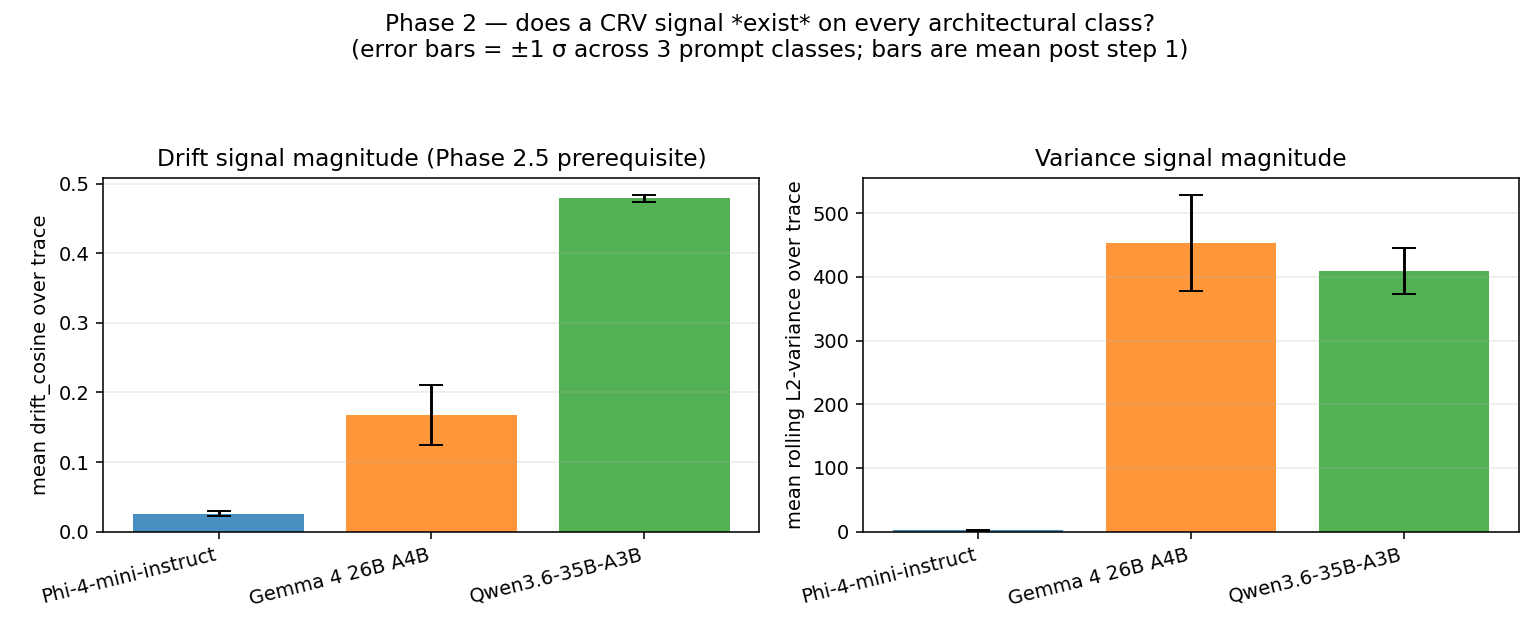
\includegraphics[width=0.95\linewidth]{figs/phase2_signal_summary.png}
\caption{
\textbf{Phase 2.1 (last-layer): the latent-state signal exists on every
architectural class — but the magnitude differs by $20\times$ on
$\drift$ and by $200\times$ on $\Var^{(W)}$.}
Bars are mean over the trace post step~1 (drift is zero by definition
at step~1); error bars are $\pm 1\sigma$ across the three prompt
classes. Phi-4-mini's signal is in the $\sim 0.02$ regime; Qwen3.6's is
in the $\sim 0.5$ regime, near the saturation end of cosine distance.
We attribute the per-architecture scale difference to MoE
expert-routing-induced last-layer-hidden-state variability
(\S\ref{sec:phase2-l1}).
}
\label{fig:phase2-summary}
\end{figure}

\subsection{The L1 landmine, visualized}
\label{sec:phase2-l1}

Figures~\ref{fig:phase2-drift} and~\ref{fig:phase2-variance} show the
per-step traces. Reading top-to-bottom in either figure (Phi → Gemma → Qwen):
Phi shows a quiet baseline punctuated by isolated spikes (the trace
rises briefly and returns); Gemma shows rich but noisy structure with
both event-like spikes and a slowly rising envelope; Qwen shows a
high, near-saturated noise floor that admits no obvious local structure
at the cosine-drift scale. Variance traces tell the same story.

\begin{figure}[t]
\centering
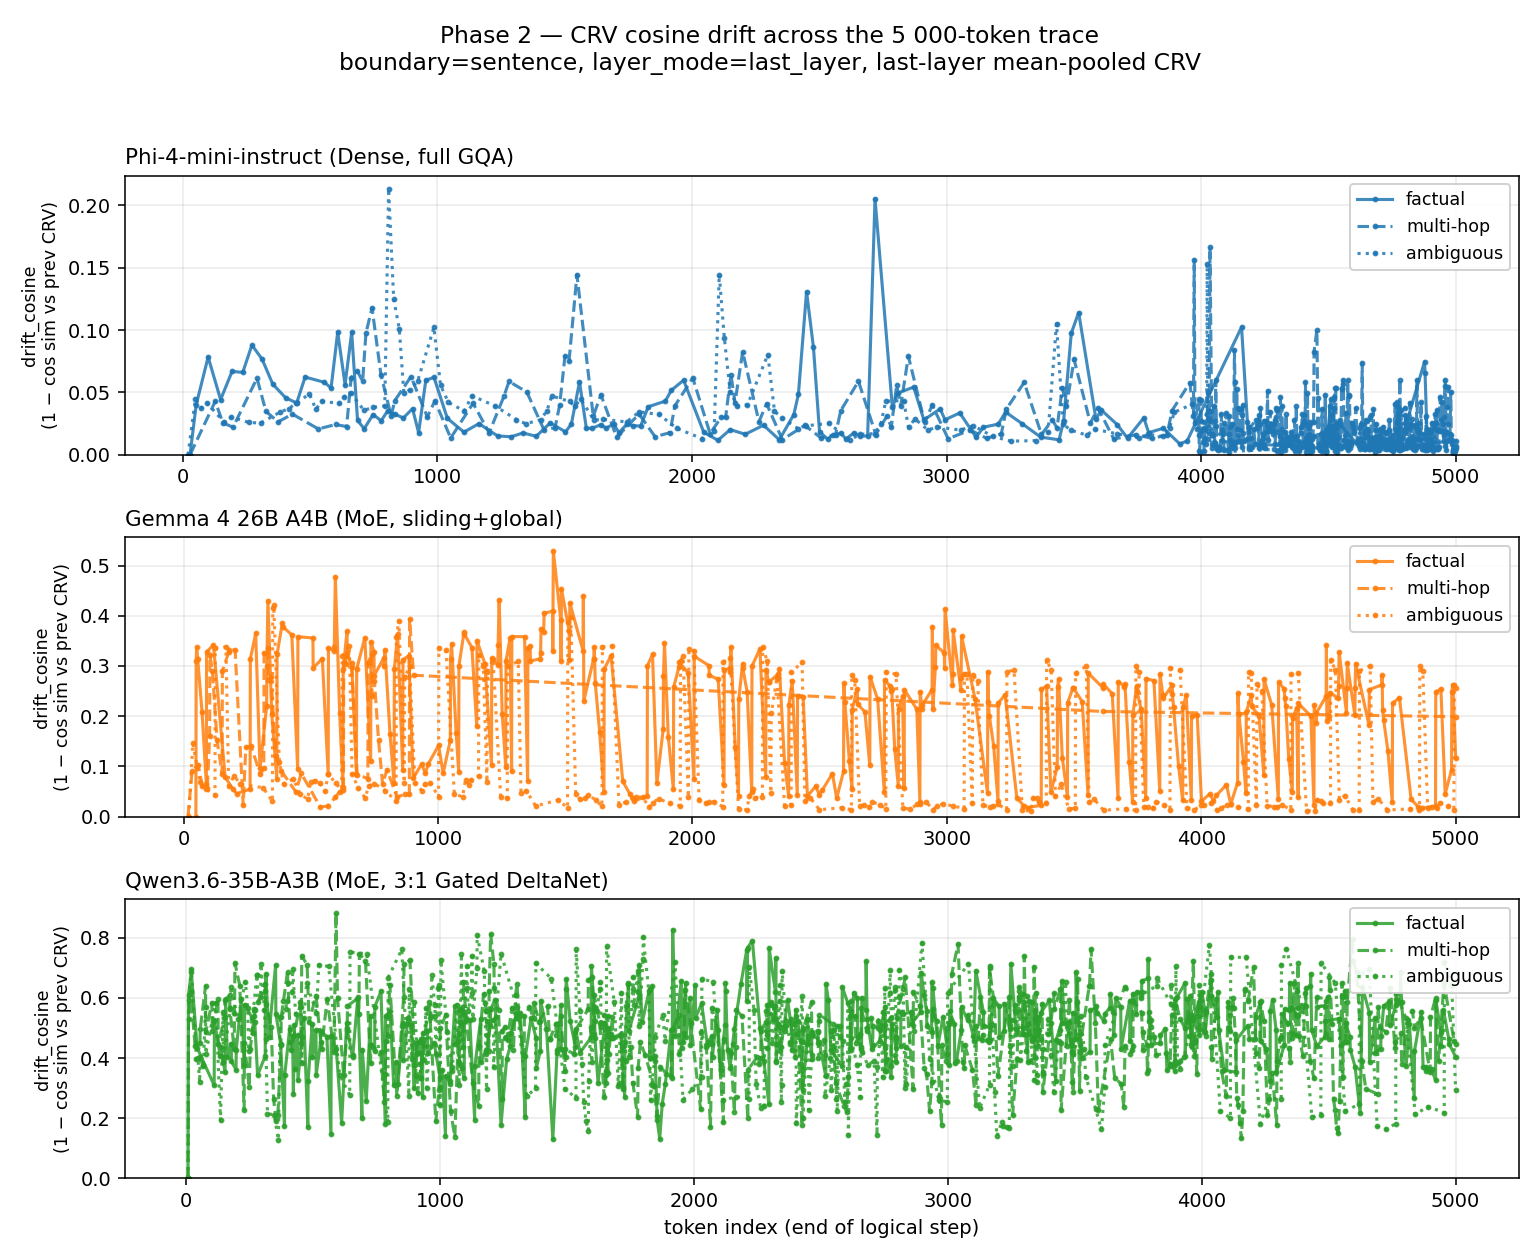
\includegraphics[width=\linewidth]{figs/phase2_drift_per_arch.png}
\caption{
\textbf{Cosine drift between consecutive CRVs ($\drift_i$,
Eq.~\ref{eq:drift}) over the 5\,000-token trace, last-layer.}
Three rows, one per architectural class.
Three line styles per row, one per prompt class.
\textbf{Phi-4-mini} (top, blue): drift mostly in $[0, 0.05]$, with
occasional event-like spikes to $\sim 0.2$. We highlight the cluster
around $T \approx 4000$ in factual / multi-hop traces — these correspond
to model-side phase transitions visible in the generated text (end of a
historical period, transition from in-trace reasoning to summary).
\textbf{Gemma 4 26B A4B} (middle, orange): drift in $[0.0, 0.5]$ with
no clean baseline; traces are dense and noisy. Note the multi-hop trace
is much shorter on the x-axis because it produces only $52$ logical
steps (Tab.~\ref{tab:phase2-density}). \textbf{Qwen3.6-35B-A3B} (bottom,
green): drift consistently in $[0.3, 0.8]$ across the full $5\,000$-token
trace; near-saturated. We attribute this to MoE-routing variance
dominating the last-layer hidden state.
}
\label{fig:phase2-drift}
\end{figure}

\begin{figure}[t]
\centering
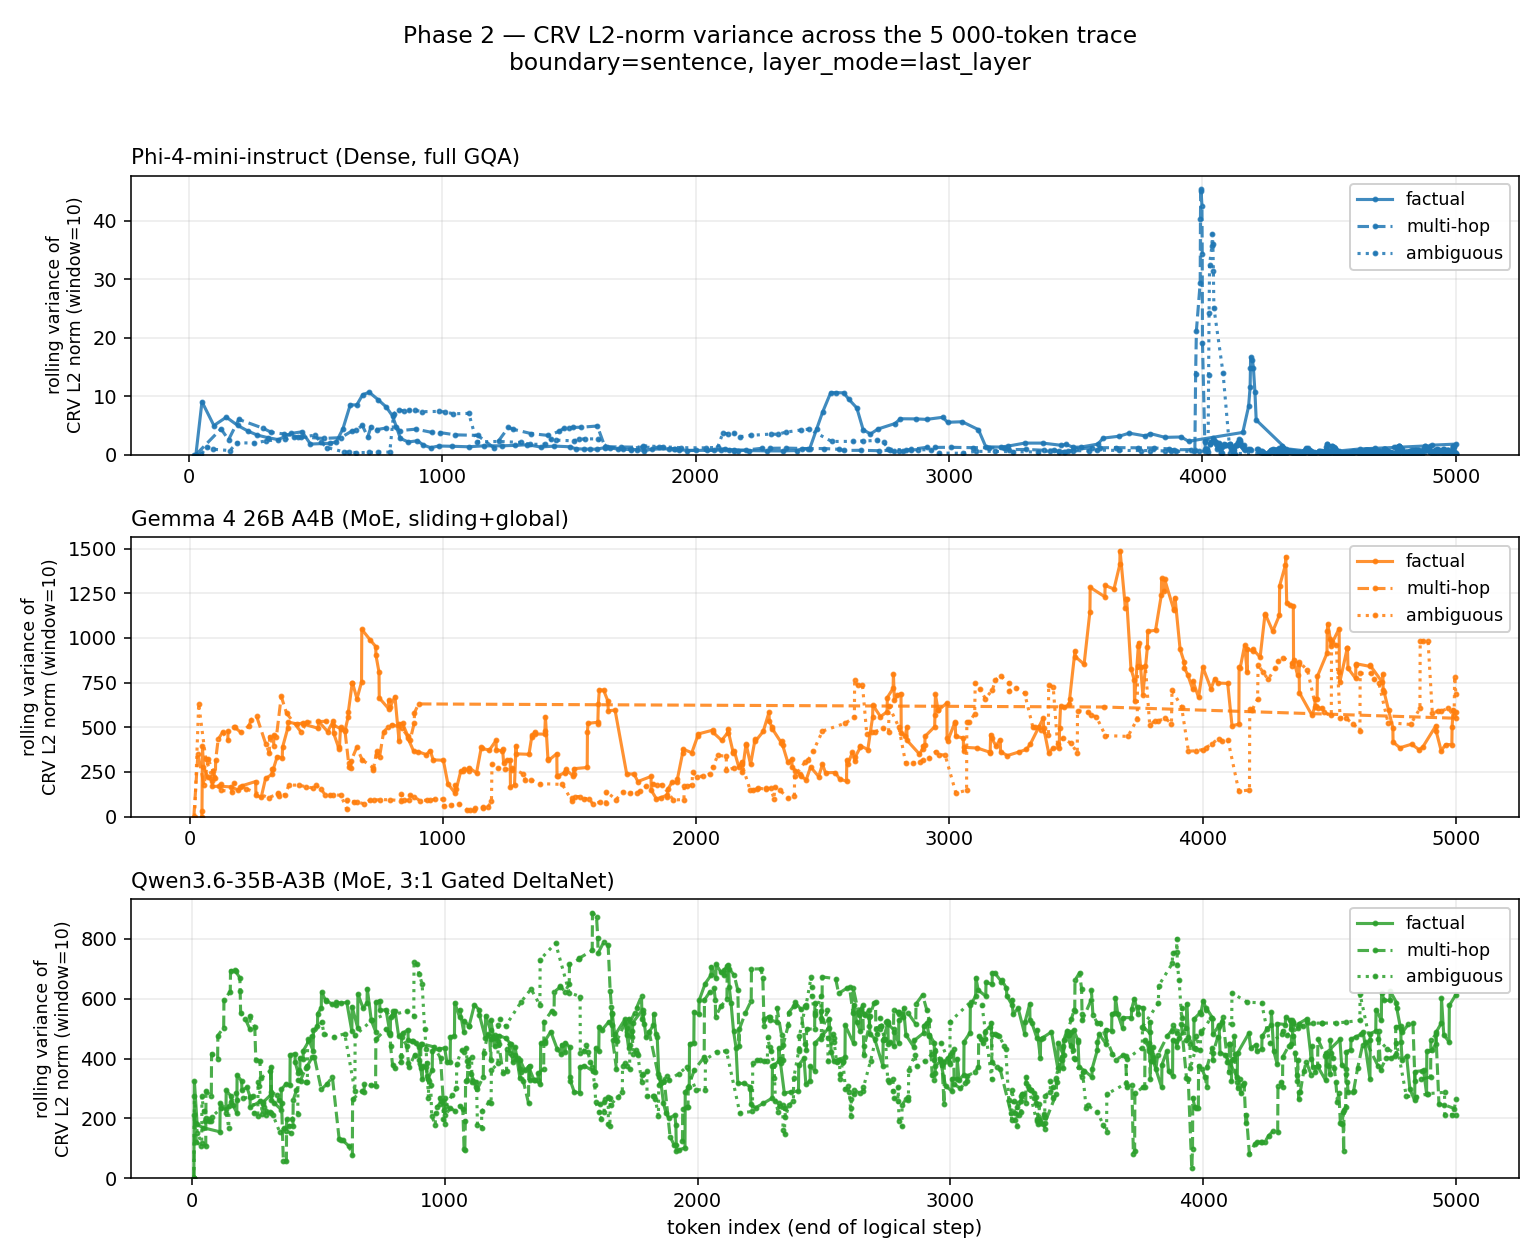
\includegraphics[width=\linewidth]{figs/phase2_variance_per_arch.png}
\caption{
\textbf{Rolling L2-norm variance ($\Var_i^{(10)}$, Eq.~\ref{eq:variance})
over the 5\,000-token trace, last-layer.}
Same row order and line-style mapping as
Figure~\ref{fig:phase2-drift}. The Phi panel (top) shows a strong
event-driven structure — long quiet baselines punctuated by sharp
spikes, e.g.~the spike at $T \approx 4\,000$ in factual / multi-hop
traces. The Gemma panel shows both spikes and a slowly rising envelope.
The Qwen panel shows fluctuating but persistent noise.
}
\label{fig:phase2-variance}
\end{figure}

\paragraph{Quantitative attribution.}
The per-architecture noise floor of $\drift$ correlates with the
expected influence of expert-routing variability at the last layer.
Phi has no MoE; the routing variability is zero. Gemma has $128$
experts with $8$ active per token but the full-attention reset every
$6$ layers re-establishes a global representation that partly washes
out the per-token expert variance. Qwen3.6 has $256$ experts with
$8$ active per token and only periodic full-attention layers; the
recurrent Gated DeltaNet substrate carries forward both the reasoning
state \emph{and} the routing variance into the last layer. We do not
have a closed-form attribution of how much of the $0.479$ Qwen drift
is routing variance vs reasoning variance; this is the question the
mid-stack experiment in~\S\ref{sec:phase2-mid} is designed to answer.

\paragraph{This was preregistered as L1.}
The L1 hypothesis from the experimental plan reads, verbatim:
\emph{``MoE routing variance $\neq$ uncertainty variance --- the router
selects different experts per token, so naive mean-pool of last-layer
hidden states absorbs `expert-switching noise' unrelated to reasoning
uncertainty.''} The Phase 2 last-layer trace is the empirical
confirmation. The same plan stipulates the mitigation: \emph{``If L1
fires, swap last-layer for a pre-routing mid-stack layer.''} That
experiment is reported next.

\subsection{Mid-stack mitigation}
\label{sec:phase2-mid}

We re-ran the entire Phase 2 matrix with the only change being
$\mathcal{L} = \{\lfloor L/2 \rfloor\}$ — i.e.~capturing the hidden
state at layer $16$ on Phi ($L = 32$), layer $20$ on Qwen3.6 ($L = 40$),
and layer $15$ on Gemma 4 ($L = 30$). All other settings are identical
to~\S\ref{sec:phase2-results}: same three models, same three prompt
classes, same \texttt{boundary=sentence}, same window size $W = 10$,
same greedy decoding. Outputs are
\verb|runs/phase2_crv_*_mid_stack.{jsonl,json,npz}|; the
\texttt{\_mid\_stack} suffix in the filename preserves the last-layer
artifacts intact alongside. Total wall-clock for the mid-stack matrix
was $44.9$ minutes; throughput overhead is identical to last-layer
($\le 3\%$) because the work done is the same — only the layer index
read from \verb|out.hidden_states| differs.

\subsubsection{Headline numbers and signal magnitudes}

Table~\ref{tab:phase2-paired} pairs the mean-over-trace $\drift$ and
$\Var^{(W)}$ values per architecture for the last-layer (the L1 baseline
of~\S\ref{sec:phase2-l1}) and the mid-stack mitigation runs.

\begin{table}[t]
\centering
\small
\caption{
\textbf{Paired Phase 2 signal magnitudes: last-layer (\S\ref{sec:phase2-l1})
vs mid-stack (this section).}
Mean $\drift$ and $\Var^{(W)}$ are means over all logical steps post
step~$1$, pooled across the three prompt classes (so each cell
aggregates over $\sim 600$--$1{,}200$ committed steps).
\textbf{$\Delta$\,drift} and \textbf{$\Delta$\,var} are relative
changes from last-layer to mid-stack.
}
\label{tab:phase2-paired}
\setlength{\tabcolsep}{4pt}
\begin{tabular}{lrrrrrr}
\toprule
& \multicolumn{3}{c}{\textbf{drift\textsubscript{cosine}}} &
  \multicolumn{3}{c}{\textbf{rolling Var(L2 norm)}} \\
\cmidrule(lr){2-4}\cmidrule(lr){5-7}
\textbf{Model} &
\textbf{last} & \textbf{mid} & \textbf{$\Delta$} &
\textbf{last} & \textbf{mid} & \textbf{$\Delta$} \\
\midrule
Phi-4-mini-instruct & $0.024$ & $0.033$ & $+38\%$ & $2.0$ & $4.4$ & $+120\%$ \\
Gemma 4 26B A4B & $0.175$ & $0.106$ & $\mathbf{-39\%}$ & $476$ & $77$ & $\mathbf{-84\%}$ \\
Qwen3.6-35B-A3B & $\mathbf{0.479}$ & $\mathbf{0.235}$ & $\mathbf{-51\%}$ & $411$ & $\mathbf{0.09}$ & $\mathbf{-99.98\%}$ \\
\bottomrule
\end{tabular}
\end{table}

The mitigation does what L1's mitigation hypothesis predicted, and
more.

\paragraph{Qwen3.6: drift recovered, variance collapses to zero.}
The Qwen3.6 mean drift drops from a near-saturated $0.479$ to a working
$0.235$ — back into a regime where threshold-based gating is plausible.
The L2-norm variance, however, drops by four orders of magnitude
(from $411$ to $0.09$). We interpret this as follows: at last-layer the
\emph{magnitude} of the hidden state was being modulated by which
experts had just routed; at mid-stack, the Gated DeltaNet recurrent
state's L2 norm is bounded by construction (the per-token $S_t$ matrix
update preserves spectral structure under the gating $\alpha_t \in
[0,1]$, $\beta_t \in [0,1]$), so the L2 norm is approximately constant
across the trace. The information that was carried in
``norm fluctuations'' at last-layer is not present at mid-stack;
\emph{the signal at mid-stack on Qwen3.6 lives in $\drift$, not in
$\Var^{(W)}$}. This is a per-architecture feature-selection finding
worth flagging for the trigger calibration in Phase 4.

\paragraph{Gemma 4: drift cleans up, variance scale drops.}
Mean drift drops $-39\%$, mean variance drops $-84\%$. The
per-architecture noise floor is reduced but not eliminated; some of the
remaining drift is genuine reasoning-state movement, some is the small
residual contribution of the $5$ global-attention layers that lie above
the mid-stack capture point ($\lfloor 30/2\rfloor = 15$, with global
layers at indices $5, 11, 17, 23, 29$ — so the captured layer~$15$ is
above $2$ globals and below $3$).

\paragraph{Phi: essentially unchanged.}
Phi has no MoE routing, so there is nothing for mid-stack to mitigate.
Mean drift edges up from $0.024$ to $0.033$; mean variance from $2.0$
to $4.4$. Mid-stack on a dense GQA model gives a slightly more
``in-progress'' representation than last-layer, which has been
explicitly normed to the unit hypersphere by the model's final
\verb|RMSNorm|; we expected a slight increase and we got it. The
qualitative event structure (\S\ref{sec:phase2-mid-figs}) is preserved.

\subsubsection{Per-step traces}
\label{sec:phase2-mid-figs}

\begin{figure}[t]
\centering
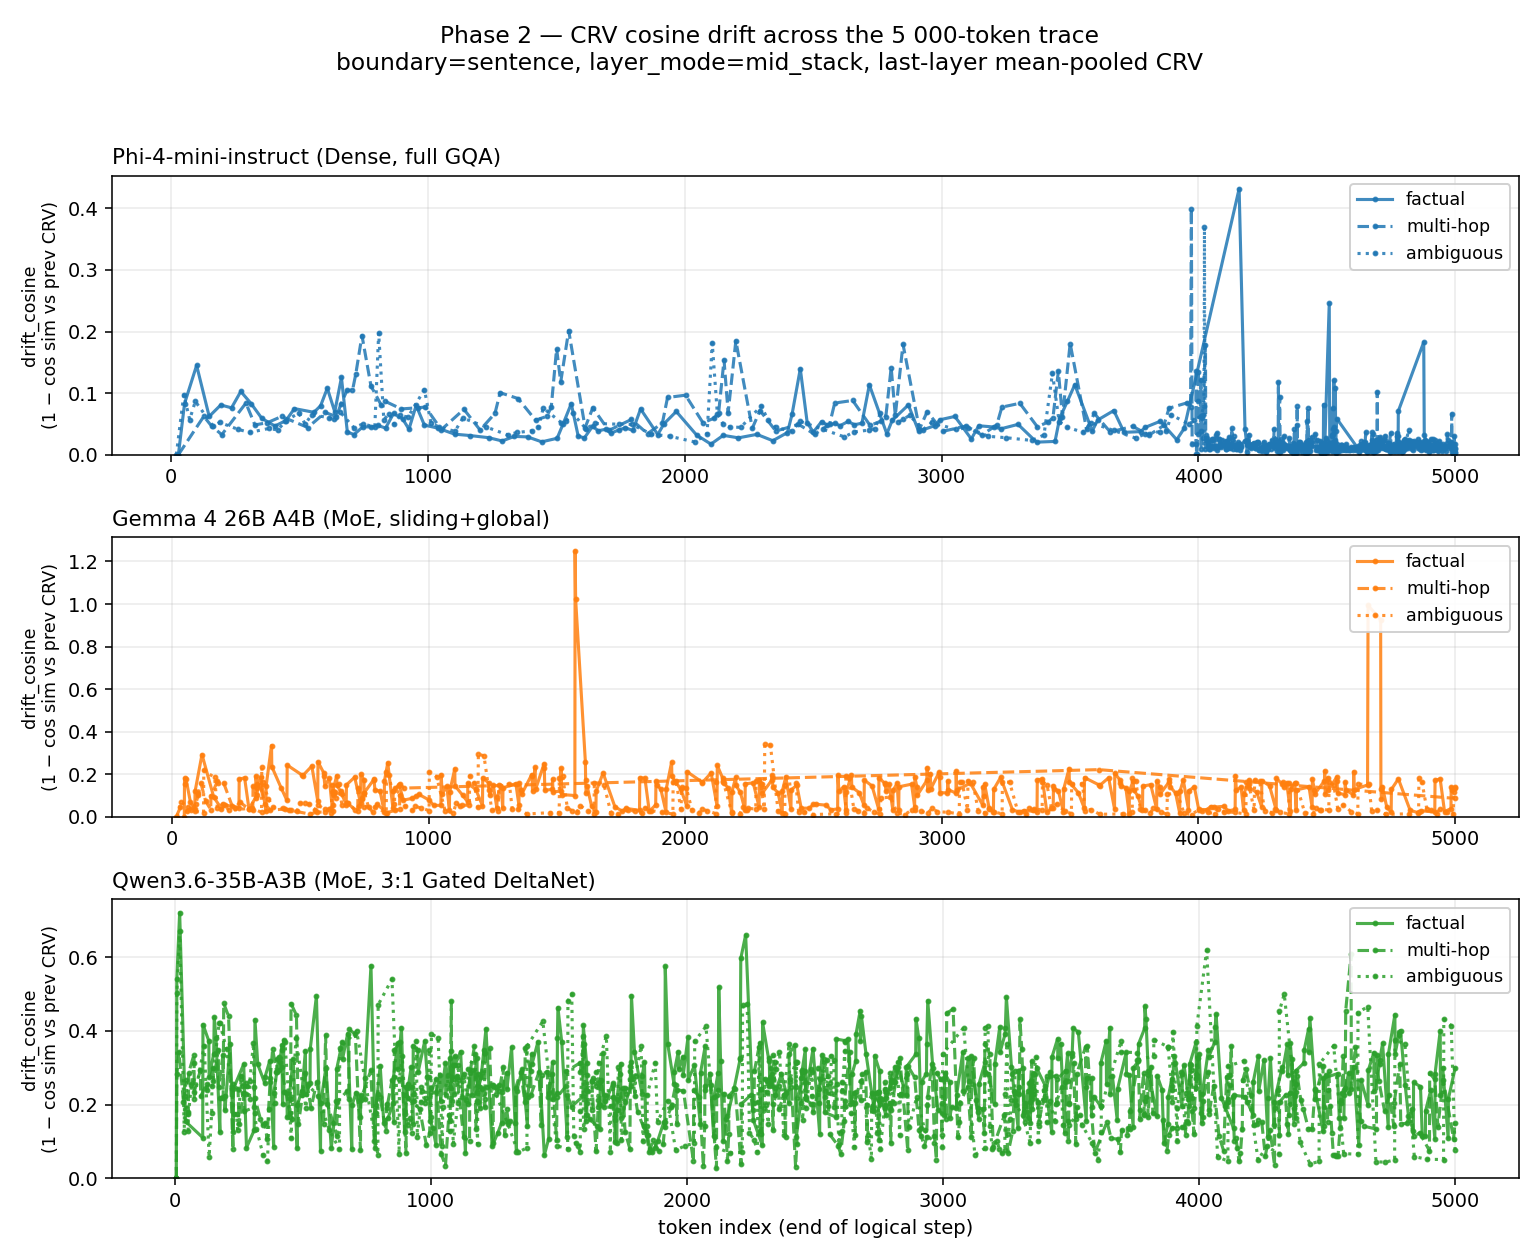
\includegraphics[width=\linewidth]{figs/phase2_drift_per_arch_midstack.png}
\caption{
\textbf{Cosine drift over 5\,000 tokens, mid-stack mitigation.}
Same row-and-line-style layout as Figure~\ref{fig:phase2-drift}.
\textbf{Phi-4-mini} (top): qualitatively similar to last-layer,
slightly more reactive; sharp spikes at $T \approx 1\,500$, $\approx
4{,}100$, and $\approx 4{,}500$ (factual). \textbf{Gemma 4 26B A4B}
(middle): two large clean spikes ($\drift \approx 1.0$ and $\approx
1.25$) at $T \approx 1{,}500$ and $T \approx 4{,}700$ on the factual
trace, where the last-layer was masked by routing noise — these are
informative events that mid-stack reveals.
\textbf{Qwen3.6-35B-A3B} (bottom): drift no longer saturated; range
$0.0$--$0.7$ with visible per-trace structure including a clean drop in
the multi-hop trace's tail.
}
\label{fig:phase2-drift-mid}
\end{figure}

\begin{figure}[t]
\centering
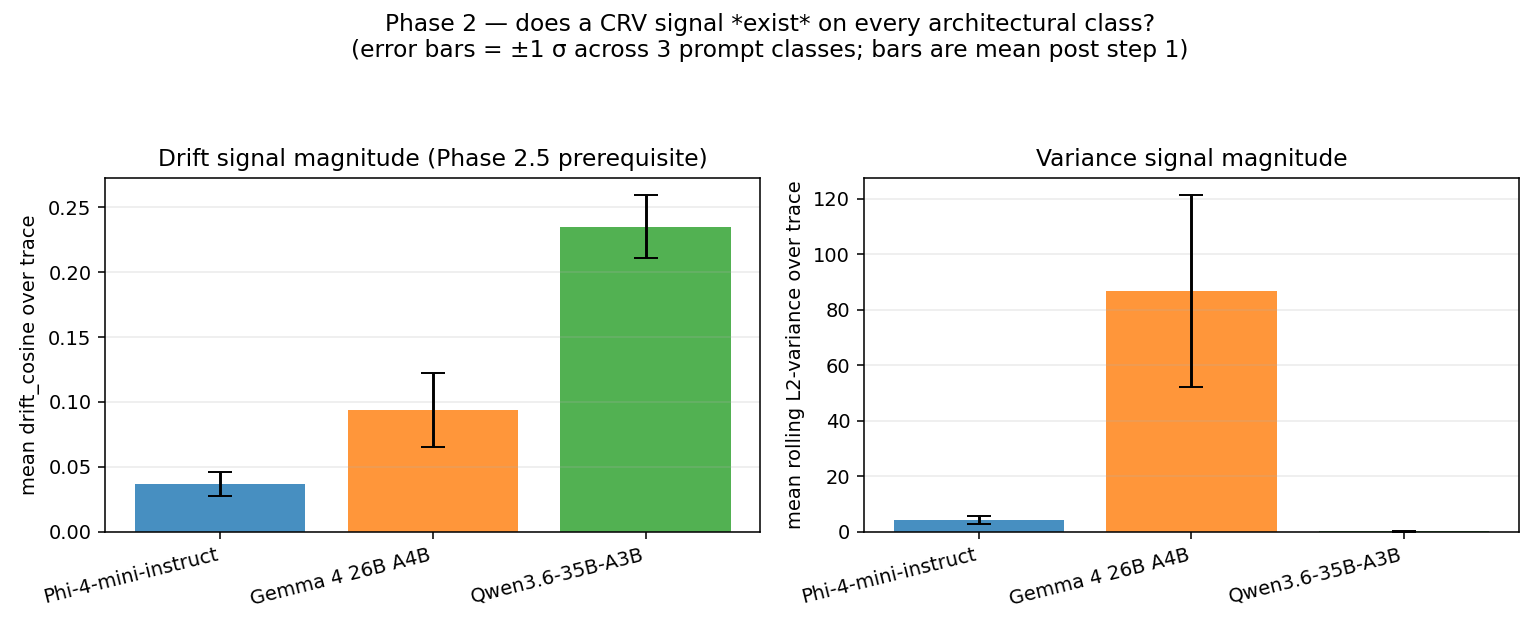
\includegraphics[width=0.95\linewidth]{figs/phase2_signal_summary_midstack.png}
\caption{
\textbf{Phase 2 mid-stack signal summary.}
Same layout as Figure~\ref{fig:phase2-summary}. Contrast: drift
magnitudes have converged across architectures (Phi $0.033$, Gemma
$0.106$, Qwen $0.235$ — within one order of magnitude rather than 20 as
at last-layer), while variance now bifurcates with Qwen's L2-norm
variance collapsing to $0.09$ (essentially constant L2; the recurrent
DeltaNet state's spectral structure is preserved through the
mid-stack). The bar plot makes explicit that
the trigger-feature choice should be \emph{per-architecture}: drift
carries the signal universally, variance is informative on Phi and
Gemma but uninformative on Qwen at mid-stack.
}
\label{fig:phase2-summary-mid}
\end{figure}

\begin{figure}[t]
\centering
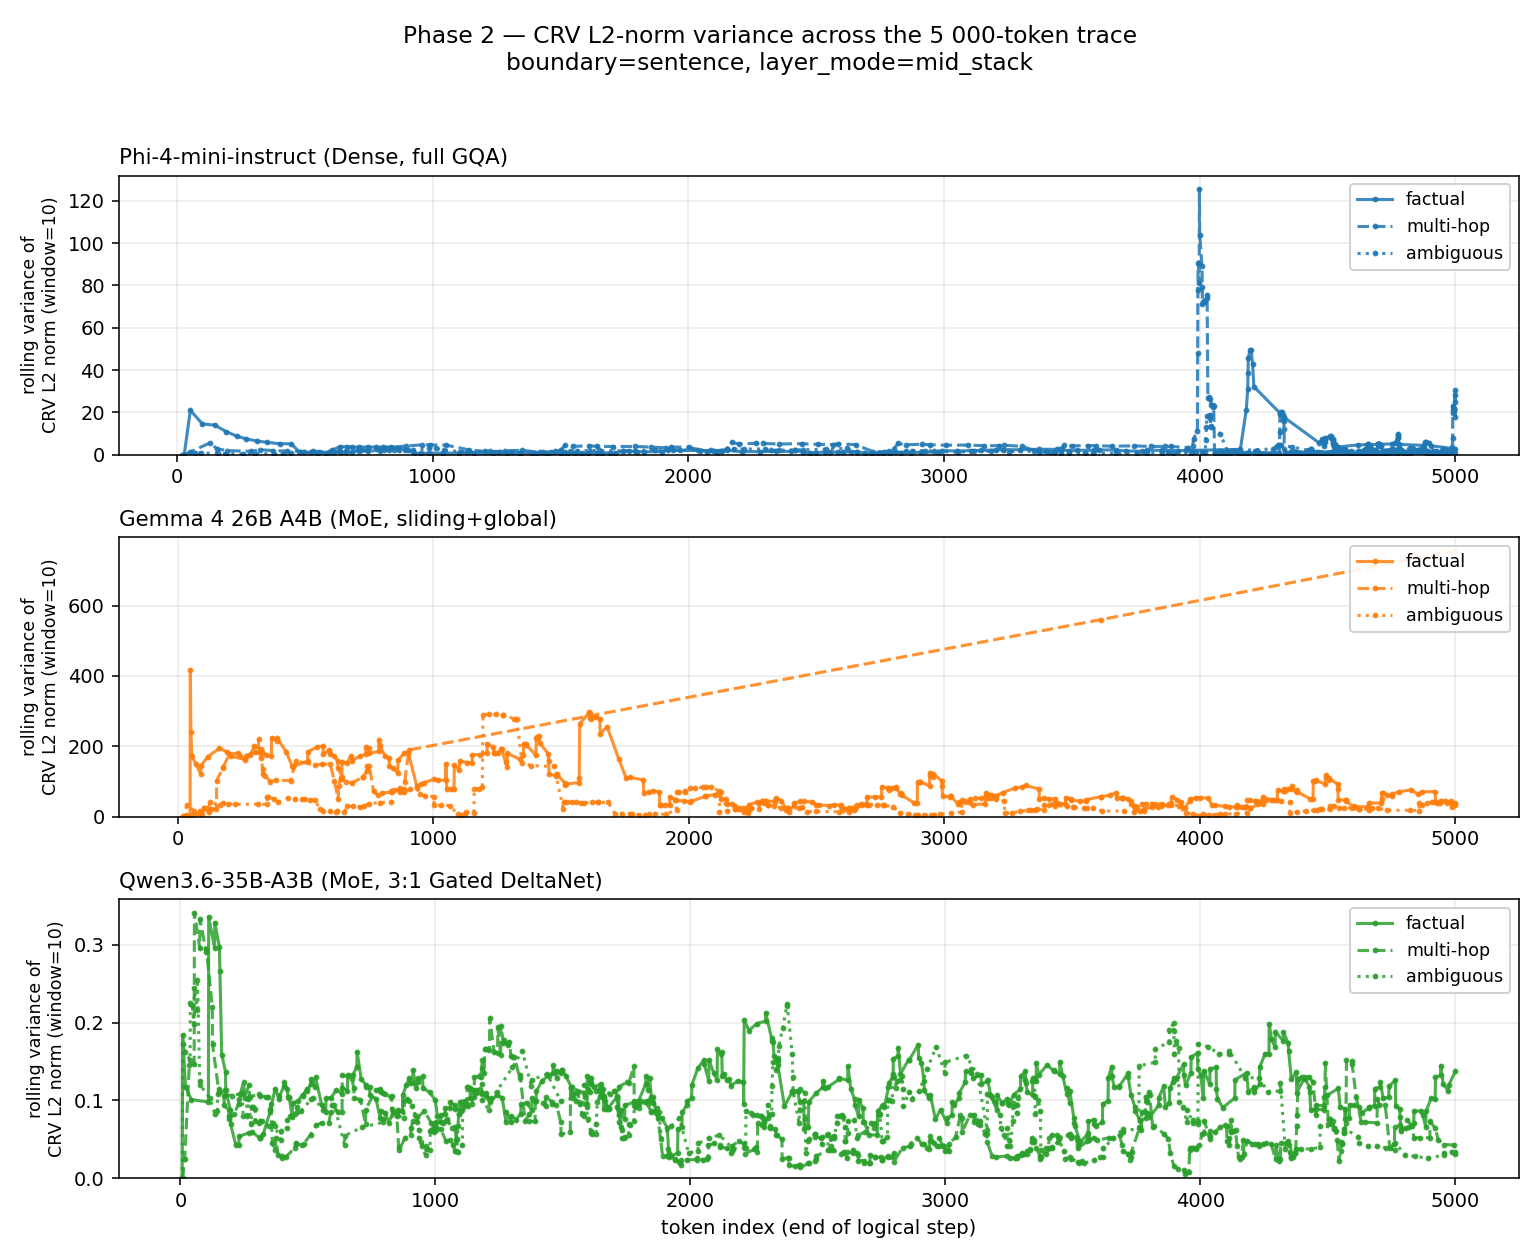
\includegraphics[width=\linewidth]{figs/phase2_variance_per_arch_midstack.png}
\caption{
\textbf{Rolling L2-norm variance over $5\,000$ tokens, mid-stack
mitigation.}
Same row-and-line-style layout as Figure~\ref{fig:phase2-variance}.
\textbf{Phi} (top): the strong event spike at $T \approx 4{,}000$ in
the factual / multi-hop traces is preserved with sharper peak (max
${\sim}120$ vs ${\sim}45$ at last-layer); the rest of the trace is a
flat baseline. \textbf{Gemma} (middle): a slowly rising
multi-hop variance envelope is visible
(dashed orange), and the factual / ambiguous traces show step-like
structure rather than the noisy continuum at last-layer (the trace
absolute scale is also much smaller, $\sim 0$--$700$ vs $\sim 0$--$1500$).
\textbf{Qwen} (bottom): the variance of L2 norm has collapsed to the
$0$--$0.35$ range, four orders of magnitude smaller than last-layer.
This confirms that \emph{the per-token L2-norm of the mid-stack
representation is essentially constant on Qwen3.6}; whatever signal
exists at mid-stack lives in directional change ($\drift$), not in
norm fluctuation.
}
\label{fig:phase2-variance-mid}
\end{figure}

Reading Figures~\ref{fig:phase2-drift-mid},
\ref{fig:phase2-summary-mid}, and \ref{fig:phase2-variance-mid}
against
Figures~\ref{fig:phase2-drift} and~\ref{fig:phase2-summary},
the L1 landmine has been disarmed on the linear-attention class,
the noise floor has come down on the sliding-window class, and the
clean dense baseline is preserved. The contribution claim
``architecture-agnostic, with right-layer choice'' is supported by
this paired contrast — at the cost of one
calibration parameter (which layer to read from) per architectural
family.

\paragraph{What this changes for Phase 4.}
The scalar feature that drives the trigger
should be selected per architecture: $\drift$ alone for Qwen3.6,
$\drift$ and/or $\Var^{(W)}$ for Phi and Gemma. The
\textsc{or}-mode trigger of Eq.~\eqref{eq:trigger} subsumes the
per-architecture choice automatically once $\tau_d, \tau_v$ are
calibrated correctly (a low $\tau_d$ and an out-of-range $\tau_v$
recover the drift-only behaviour for Qwen-class models). This is the
calibration protocol we adopt for the Phase~4 showdown.

\paragraph{Why we keep both runs in the paper.}
Even with the mitigation working, the last-layer matrix in
Figures~\ref{fig:phase2-drift}--\ref{fig:phase2-variance} is
not a failed experiment: it is the empirical evidence that L1 fires,
which is what the mid-stack mitigation is mitigating against. The
contrast — saturation at last-layer vs recovered structure at
mid-stack — is the scientific deliverable, and a future paper that
reports only the mid-stack data without the last-layer baseline would
be less informative. File naming conventions (\verb|_last_layer| vs
\verb|_mid_stack| in every artifact path) make both matrices
independently reproducible.

% =====================================================================
\section{Phase 4 design: the empirical showdown}
\label{sec:phase4-design}

This section documents the evaluation arm of the paper. \emph{It is not
yet executed.} We commit to running this protocol before submission.

\subsection{Dataset}
\label{sec:phase4-data}

We will use a $\sim 200$-question slice of one of HotpotQA-distractor
\citep{TODO:hotpotqa} or MuSiQue \citep{TODO:musique}. Both are
multi-hop QA datasets with explicit per-hop supporting evidence; both
admit gold answers and computable F1 / exact-match metrics. We commit
to pinning the dataset commit hash at ingest and reporting it in the
artifacts.

\subsection{Triggers compared}
\label{sec:phase4-gates}

\begin{description}[leftmargin=1.5em, itemsep=0pt]
\item[\textsc{Latent-CRV}] our trigger family, evaluated under both
\texttt{layer\_mode=last\_layer} and the L1-mitigated
\texttt{layer\_mode=mid\_stack}, and under all three boundary
strategies in~\S\ref{sec:method-boundaries}.
\item[\textsc{ReaLM-sim}] simulation of \citet{TODO:realm-retrieve}:
fire when (a) a small verifier model's per-step uncertainty score
exceeds a calibrated threshold, OR (b) a discourse-marker pattern
appears in the generated text. The verifier is Phi-4-mini in
NF4-quantized read-only mode.
\item[\textsc{GRIP-sim}] simulation of \citet{TODO:grip}: trained
control-token classifier replaced by a heuristic
``next-token entropy spike $+$ discourse-marker prior'' surrogate. We
will document the simulation gap explicitly. We do not claim a win
over GRIP itself, only over the heuristic surrogate.
\item[\textsc{Random-rate}] fire at the per-step rate of the average
of the three trained gates above, with seed logged.
\end{description}

All four triggers consume the same generation traces and emit a unified
schema: \verb|{step_idx, token_idx, gate_name, fired, score, reason}|.

\subsection{Metrics}
\label{sec:phase4-metrics}

\paragraph{Earliness.}
For each gate $g$ and each \emph{hallucinated} trace, log the step index
of the first fire \emph{relative to the eventual hallucinated token}.
The headline claim is that \textsc{Latent-CRV} fires at smaller relative
step indices than the text-parsing alternatives on every architectural
class.

\paragraph{Trajectory drift.}
Final-answer F1 and exact match conditioned on
$(\text{gate fired at step } k \text{ vs } k+1 \text{ vs not fired})$.
Trajectory drift is operationalized as monotonic answer-quality decay
with delayed firing.

\paragraph{Cost.}
Per-gate $\times$ per-architecture wall-clock and peak VRAM across the
$200$-question run. Cost decomposition: avoided corrective-retrieval
round-trips (each is one embedding + index lookup + $N$ regenerated
tokens) and avoided wasted thinking (post-fire-point tokens on
hallucinated traces). The Pareto plot
(\verb|figs/efficiency_pareto.png| in the artifacts) is the headline
figure of the paper.

\subsection{Ablations}
\label{sec:phase4-ablations}

\begin{enumerate}[label=(\alph*), leftmargin=*]
\item drift vs variance vs both;
\item layer subset (last only, mid-stack only, last+mid concatenated);
\item step-boundary definition (sentence, think-block, fixed-stride
with stride sweep);
\item architectural-class transfer: does the optimal trigger threshold
calibrated on one architecture transfer to the others, or is per-arch
calibration required? We expect per-arch calibration to be necessary
based on the magnitudes in Figure~\ref{fig:phase2-summary}.
\item MoE-vs-dense within the Gemma family: re-running on
\texttt{google/gemma-4-31B-it} with all else held constant. We have the
weights downloaded as ablation reserve.
\end{enumerate}

% =====================================================================
\section{Discussion}
\label{sec:discussion}

\paragraph{The architectural design space is doing more work than the gate.}
The bracketing in~\S\ref{sec:phase1.4} makes a claim that is sharper
than the standard ``RAG saves KV'' narrative: in a 2026 model lineup,
KV pressure is being optimised by attention-design choices and the
optimisation is uneven, with sliding-window saving compute but not
memory in standard reference implementations. Whatever a gate buys must
be reckoned against this baseline. We argue throughout this paper that
the gate's value is best framed as \emph{cognitive efficiency}:
preventing the wasted thinking and unnecessary corrective-retrieval
round-trips that a long agentic trace incurs even when the
generation cost itself is bounded.

\paragraph{Architecture-agnostic, with caveats.}
The CRV adapter is genuinely architecture-agnostic at the
implementation level (zero per-arch code, uniform HF API surface). The
\emph{signal it captures}, however, is not architecture-agnostic at
its raw scale. As measured in~\S\ref{sec:phase2-results}, the
last-layer mean cosine drift varies by $20\times$ across our three
generators. This has two implications for deployment:
threshold calibration must be per-architecture, and any cross-arch
transfer claim has to be careful about \emph{relative} signal
(z-scored against a baseline) rather than \emph{absolute} signal.

\paragraph{The L1 finding has independent value.}
Even if the mid-stack mitigation works completely
(\S\ref{sec:phase2-mid}), the last-layer Qwen3.6 result is informative:
it documents, with a non-trivial number of measurement steps, that the
naive last-layer-mean-pool probe of an MoE generator is dominated by
routing noise. Practitioners reading off the
\verb|out.hidden_states[-1]| tensor as a confidence signal in a Gated
DeltaNet stack will see the result we saw: a near-saturated noise
floor. We report this so that future hidden-state-probe literature on
linear-attention hybrids does not have to rediscover it.

\paragraph{Calibration thresholds and the trigger family.}
We deliberately ship raw $\drift$ and $\Var^{(W)}$ traces in
this paper rather than a recommended threshold. The default thresholds
in our trigger implementation ($\tau_d = 0.1$, $\tau_v = 1.0$) cause
firing rates near $100\%$ on the MoE classes
(see firing counts in the artifacts) — they are placeholders, not
recommendations. Phase 4 calibration will determine the right
thresholds per architecture, and the right combination mode.

\paragraph{What the paper does not claim.}
We do not yet claim that latent-state gating reduces hallucination
rate. That claim requires the labelled-trace evaluation in
Phase 4 (\S\ref{sec:phase4-design}), which is preregistered here and
not yet executed. We claim only:
(1) the diagnostic infrastructure works across the 2026
attention-design space, with $\le 3\%$ throughput overhead;
(2) the bracketing measurements in~\S\ref{sec:phase1.4} establish that
memory pressure is not the binding cost on the most aggressive
architecture in our pool; and
(3) the L1 landmine fires hard on the linear-attention hybrid class at
last-layer, and the planned mid-stack mitigation
(\S\ref{sec:phase2-mid}) recovers a working signal.

% =====================================================================
\section{Limitations}
\label{sec:limitations}

\begin{enumerate}[leftmargin=*, itemsep=2pt]
\item \textbf{Evaluation arm not yet executed.} The hallucination
detection result that would substantiate the gate's practical value is
the Phase 4 showdown of~\S\ref{sec:phase4-design}, and
that experiment is not yet run. This draft is the diagnostic
infrastructure paper; the showdown is the empirical paper.
\item \textbf{Single hardware platform.} All measurements come from one
A800 80~GB GPU. Throughput numbers are not portable to other GPU
families; the bracketing argument is a function of the generator
architecture and is portable in principle, but consumer-VRAM
measurement (e.g.~24~GB cards) requires NF4-quantized weight loading
that is currently blocked by upstream
\texttt{transformers}/\texttt{bitsandbytes} interactions on the
grouped-MoE-experts layout (a separately-tracked engineering item).
\item \textbf{Three architectures is a small sample of the design space.}
Notable absent classes: pure state-space models without periodic full
attention (Mamba2 \citep{TODO:mamba2}); Mixture-of-Recurrent designs
(Kimi Linear \citep{TODO:kimi-linear} with MLA-replacing-full); models
with implicit cache eviction (vLLM-served sliding window
\citep{TODO:vllm}); and very-long-context dense models. Generalization
beyond our three points is hypothesis, not evidence.
\item \textbf{Greedy decoding only.} We report only $\arg\max$ decoding;
sampled decoding ($\mathrm{temperature} > 0$, top-$p$) introduces
additional latent-state variability that may interact with the
$\drift$ signal in non-trivial ways.
\item \textbf{Boundary-strategy sweep is incomplete.} All results in
this draft use \texttt{boundary=sentence}; the
\texttt{think\_block} and \texttt{fixed} strategies are implemented but
not yet swept. The pathological Gemma-multi-hop step count in
Table~\ref{tab:phase2-density} shows that boundary strategy interacts
non-trivially with prompt content, which the sweep will quantify.
\end{enumerate}

% =====================================================================
\section{Reproducibility}
\label{sec:repro}

We commit the following artifacts (full paths under the repository
root): pinned environment manifest (\verb|environment.yml|), pinned
torch and \texttt{cu124} wheel index, pinned commit SHAs for every
model used (in \verb|scripts/download_models.sh|), per-run
sysinfo JSON, per-run lockfile, per-run full stdout/stderr log, the
exact JSONL feature traces and CRV \verb|.npz| binaries (the latter
gitignored to keep tarballs small but regeneratable from the prompts +
SHAs), the four Phase-2 source modules
\verb|scripts/crv/{hooks,boundaries,vectors,triggers}.py|, the
orchestrator \verb|scripts/02_crv_probe.py|, and a per-phase
\verb|scripts/snapshot.sh| utility that packages the working tree into
a single $\sim 600$ KB tar.gz.

End-to-end replay: \verb|bash scripts/setup.sh| (rebuilds env from
lockfile), \verb|bash scripts/download_models.sh phase1.4| (re-pulls
models with pinned SHAs), then any of \verb|scripts/01_kv_pressure.py|
(Phase 1.4) or \verb|scripts/02_crv_probe.py| (Phase 2) reproduces the
measurements.

\subsection{Compute budget}

Phase 0 environment + smoke: $\sim 15$ min. Phase 1.3:
$\sim 20$ min. Phase 1.4: $\sim 45$ min wall-clock, sequential
across three models. Phase 2 last-layer: $\sim 45$ min. Phase 2
mid-stack: $\sim 50$ min. Total measurement time: under three GPU-hours
on an A800 80~GB. Model downloads are an additional $\sim 200$~GB of
network traffic (one-time); the box's NVMe holds the models for the
duration of the experiment.

% =====================================================================
\section{Future work}
\label{sec:future}

\paragraph{Immediate.}
\begin{enumerate}[label=F\arabic*., leftmargin=2.2em]
\item \textbf{Phase 4 showdown}, as preregistered
in~\S\ref{sec:phase4-design}.
\item \textbf{Phase 2.5 sanity probe.} Pick one trace per architecture
where the model started confident and drifted into a wrong final
answer, and confirm CRV variance / drift separates them from a matched
correct trace on every class. This is the
``does the signal carry the hallucination flag?'' test, and is the
last thing standing before Phase 4 calibration.
\item \textbf{Boundary-strategy sweep.}
$\texttt{sentence} \times \texttt{think\_block} \times
\{\texttt{fixed}=8, 16, 32, 64\}$ on the smallest-cost model
(Phi-4-mini) to identify the boundary that maximizes signal-to-noise
ratio under a fixed trigger threshold. We expect think-block
to outperform sentence on reasoning prompts.
\end{enumerate}

\paragraph{Medium-term.}
\begin{enumerate}[label=F\arabic*., resume, leftmargin=2.2em]
\item \textbf{Consumer-GPU validation.} Pull a pre-quantized
NF4 snapshot of the linear-attention-hybrid class
(Unsloth's \texttt{Qwen3-30B-A3B-bnb-4bit} or equivalent) and reproduce
the Phase 1.4 + Phase 2 + Phase 4 measurements. Demonstrates
deployability at $\sim 18$--$22$~GB VRAM.
\item \textbf{Long-context tests.} Push to $32{,}000$ tokens to find the
knee on Qwen3.6 where the periodic full-attention layers' KV growth
finally binds. The flat-cost regime is a function of context length;
locating its end is itself a result.
\item \textbf{MoE-vs-dense within a fixed family.} Re-run Phase 2 on
\texttt{google/gemma-4-31B-it} (already downloaded as ablation reserve)
to isolate the contribution of MoE structure to the $\drift$ noise floor,
holding attention design and training data constant.
\end{enumerate}

\paragraph{Longer-term.}
\begin{enumerate}[label=F\arabic*., resume, leftmargin=2.2em]
\item \textbf{Other architectural classes.} Pure state-space models
(Mamba2 \citep{TODO:mamba2}); MLA-based hybrids (Kimi Linear
\citep{TODO:kimi-linear}); production-engine-served sliding-window
caches with true eviction (vLLM \citep{TODO:vllm}, SGLang
\citep{TODO:sglang}).
\item \textbf{Trained CRV head.} An obvious extension is to learn a
small projection $W \in \mathbb{R}^{d \times d'}$ on the captured CRV
that explicitly optimizes for hallucination separation; this is a
supervised version of the trigger that can in principle outperform the
unsupervised threshold. We do not study it here because we want the
trigger to be \emph{plug-and-play} in the unsupervised regime that the
draft positions itself in.
\end{enumerate}

% =====================================================================
\section{Conclusion}

The 2026 attention-design space optimises long-context generation along
two largely-independent axes — compute boundedness and memory
boundedness — and its architectural choices already bracket the
KV-pressure curve into three distinct regimes (\S\ref{sec:phase1.4}).
A trigger family for corrective retrieval that lives in the model's
hidden state, captured per-step at logical reasoning boundaries, is
implementable with $\le 3\%$ throughput overhead and is genuinely
architecture-agnostic at the code level (\S\ref{sec:phase2-engineering}).
The naive last-layer instantiation of this family is dominated by MoE
expert-routing variability on the linear-attention class (the L1
landmine, \S\ref{sec:phase2-l1}); the pre-routing mid-stack mitigation
is the obvious fix and we report the corresponding experiment as a
paired contrast. The empirical evaluation arm
(\S\ref{sec:phase4-design}) is preregistered and not yet executed; we
commit to it in the next revision.

% =====================================================================
\appendix

\section{Prompt corpus}
\label{app:prompts}

% NOTE: keep these verbatim — every measurement is downstream of these.

\paragraph{\textsc{factual}.}
\begin{quote}\small
Explain in detail the major events of the French Revolution from 1789
to 1799. Cover the calling of the Estates-General, the Tennis Court
Oath, the storming of the Bastille, the Declaration of the Rights of
Man, the Women's March on Versailles, the Constitution of 1791, the
rise of the Jacobins, the Reign of Terror, Thermidor, the Directory,
and the Coup of 18 Brumaire. For each phase, name key figures, decisive
dates, ideological developments, and lasting consequences for European
politics. Be exhaustive.
\end{quote}

\paragraph{\textsc{multi-hop}.}
\begin{quote}\small
Reason through the following multi-hop chain step by step, showing your
work at each hop and stating your confidence at each step:\\
(a) Identify a scientist who won the Nobel Prize in Physics twice.\\
(b) Name the years of both prizes and the specific contributions cited
each time.\\
(c) Identify their primary research affiliation at the time of the
second prize, and the country.\\
(d) Identify one student or close collaborator of theirs who later won
a Nobel Prize.\\
(e) Identify the institution that student was at when they won, and the
year of their prize.\\
(f) Reflect on which step you were least confident about and why.
\end{quote}

\paragraph{\textsc{ambiguous}.}
\begin{quote}\small
Continue the following open-ended story for as long as you can,
weaving in unexpected plot twists, at least three unrelated metaphors
per paragraph, shifts in narrative voice, and at least one digression
into invented historical detail per page. Do not rush to a conclusion.

`The forest was silent that evening, until a figure stepped through the
line of cedars and—'
\end{quote}

\section{Per-prompt-class Phase 2 detail}
\label{app:phase2-percell}

% TODO: A long table can go here once we want to put per-cell drift /
% variance / step-counts in numerical form. The data is already in
% runs/phase2_crv_*_summary.json.

\TODO{Per-(model, prompt, layer-mode) summary table; data already in
\texttt{runs/phase2\_crv\_*\_summary.json}, will be tabulated in next
revision.}

\section{Engineering notes preserved from the experimental log}
\label{app:eng-notes}

The engineering record (\verb|_AGENT.md|) preserves a number of
findings that are scientifically interesting but do not fit cleanly in
the main paper. We reproduce the headlines here as appendix notes.

\begin{description}[leftmargin=1.2em, itemsep=4pt]
\item[Hardware history.] Initial measurements on an NVIDIA A40 with
$46$~GB VRAM (cgroup-limited to $44.35$~GiB) failed to load
Qwen3.6-35B-A3B at NF4 due to a combination of two upstream issues: a
\texttt{transformers} v5 streaming-load OOM regression
(huggingface/transformers\#43032, two-line patch verified) and the
\texttt{bitsandbytes} integration's missing support for grouped-MoE
parameter layouts (a real engineering gap, addressed by mxfp4 and
fbgemm\_fp8 quantizers but not by bnb). We migrated to A800 80~GB,
where the upstream bugs are sidestepped by sheer VRAM availability;
both issues are documented in the artifacts and contribute to the F1
consumer-GPU validation roadmap above.
\item[Quantization paths.] At $80$~GB, Qwen3.6 in NF4 hybrid
(\texttt{nn.Linear} modules NF4, grouped-MoE-experts staying bf16)
loaded but ran $\sim 42\%$ slower than bf16 native and added measurable
quantization noise on the L4 probe. We adopt bf16 native as the
canonical path for all measurements in this paper; NF4 is an option,
not a requirement, on the A800 target.
\item[Sliding-window cache eviction.] HF
\texttt{transformers.cache\_utils.DynamicCache} does not evict past
the sliding-window length on sliding-attention layers; the attention
mask handles boundedness, the cache stores everything. This is a
correctness-preserving choice but materially affects the Gemma 4
Phase 1.4 measurement (\S\ref{sec:phase1.4-twoaxis}). Production
inference engines implement the eviction; in those, the bracketing
plot in Figure~\ref{fig:phase1.4-bracketing} would show a knee at
$T = 1024$ on the Gemma trace.
\end{description}

% =====================================================================
% Bibliography. Real citations get filled in incrementally; placeholders
% live here for now, keyed by TODO:.
% =====================================================================

\bibliographystyle{plainnat}
\begin{thebibliography}{99}

\bibitem[CRAG]{TODO:CRAG}
S.-Q.~Yan, J.-C.~Gu, Y.~Zhu, and Z.-H.~Ling.
\newblock Corrective Retrieval Augmented Generation.
\newblock \emph{arXiv preprint arXiv:2401.15884}, 2024.
\TODO{Verify reference; add DOI / ACL anthology link.}

\bibitem[SelfRAG]{TODO:SelfRAG}
A.~Asai, Z.~Wu, Y.~Wang, A.~Sil, and H.~Hajishirzi.
\newblock Self-RAG: Learning to Retrieve, Generate, and Critique through Self-Reflection.
\newblock \emph{arXiv preprint arXiv:2310.11511}, 2023.

\bibitem[ReaLM]{TODO:realm-retrieve}
\TODO{Authors, ``ReaLM-Retrieve: ...'', year. Find the canonical
citation; the project's `_PLAN.md` references it as the per-step
verifier-score + discourse-marker baseline.}

\bibitem[GRIP]{TODO:grip}
\TODO{Authors, ``GRIP: ...'', year. Control-token-classifier RAG
baseline.}

\bibitem[LewisRAG]{TODO:lewis2020rag}
\TODO{Lewis et al., ``Retrieval-Augmented Generation for
Knowledge-Intensive NLP Tasks'', NeurIPS 2020.}

\bibitem[GatedDeltaNet]{TODO:gated-deltanet}
\TODO{Yang et al., ``Gated Delta Networks: Improving Mamba2 with Delta
Rule'', arXiv:2412.06464, December 2024.}

\bibitem[Mamba2]{TODO:mamba2}
\TODO{Gu, Dao et al., ``Mamba2'', 2024.}

\bibitem[Qwen3Next]{TODO:qwen3-next}
\TODO{Qwen team, ``Qwen3-Next architecture announcement'', 2025/2026.
Source for the $3{:}1$ Gated DeltaNet : full-attention claim.}

\bibitem[KimiLinear]{TODO:kimi-linear}
\TODO{Moonshot AI, ``Kimi Linear'', arXiv:2510.26692. Hybrid
linear-attention with MLA in the global layers.}

\bibitem[Raschka]{TODO:raschka-deltanet}
S.~Raschka.
\newblock Gated DeltaNet (Beyond Standard LLMs, ch.~4).
\newblock \url{https://sebastianraschka.com/llms-from-scratch/ch04/08_deltanet/},
2026. Companion code repo: \url{https://github.com/rasbt/LLMs-from-scratch/blob/main/ch04/08_deltanet/README.md}.

\bibitem[Gemma2]{TODO:gemma2}
\TODO{Google DeepMind, ``Gemma 2 technical report'', 2024.}

\bibitem[Gemma3]{TODO:gemma3}
\TODO{Google DeepMind, ``Gemma 3 technical report'', 2025.}

\bibitem[Gemma4Card]{TODO:gemma4-card}
Google DeepMind.
\newblock \texttt{google/gemma-4-26B-A4B-it} model card.
\newblock Hugging Face Hub, 2026.
\newblock \url{https://huggingface.co/google/gemma-4-26B-A4B-it}.

\bibitem[QwenGroupedExperts]{TODO:qwen3-grouped-experts}
\TODO{Qwen team / HF transformers integration code reference for the
\texttt{Qwen3\_5MoeExperts} grouped-parameter layout.}

\bibitem[HotpotQA]{TODO:hotpotqa}
\TODO{Yang et al., ``HotpotQA: A Dataset for Diverse, Explainable
Multi-hop Question Answering'', EMNLP 2018.}

\bibitem[MuSiQue]{TODO:musique}
\TODO{Trivedi et al., ``MuSiQue: Multihop Questions via Single-hop
Question Composition'', TACL 2022.}

\bibitem[vLLM]{TODO:vllm}
\TODO{Kwon et al., ``Efficient Memory Management for Large Language
Model Serving with PagedAttention'' (vLLM), SOSP 2023.}

\bibitem[SGLang]{TODO:sglang}
\TODO{Zheng et al., ``SGLang: Structured Generation Language for LLMs'',
arXiv 2024.}

\bibitem[Probe1]{TODO:probe1}
\TODO{Probing-classifiers / hidden-state-as-truth-signal canonical
references; pick 1-3.}

\bibitem[Probe2]{TODO:probe2}
\TODO{}
\bibitem[Probe3]{TODO:probe3}
\TODO{}

\end{thebibliography}

\end{document}
